% This is samplepaper.tex, a sample chapter demonstrating the
% LLNCS macro package for Springer Computer Science proceedings;
% Version 2.20 of 2017/10/04
%
\documentclass[runningheads]{llncs}
\usepackage{amsmath}
\usepackage{amssymb}
\usepackage{mathrsfs}
\usepackage{graphicx}
\usepackage{subfigure}
\usepackage{physics}
\usepackage{tikz} 
\usepackage{scalefnt}
\usepackage{qcircuit}
\usepackage{tabularx} 
\usepackage{float}
\usepackage{enumerate}
\usepackage{multirow}

\usepackage[linesnumbered,ruled,lined]{algorithm2e}
% Used for displaying a sample figure. If possible, figure files should
% be included in EPS format.
%
% If you use the hyperref package, please uncomment the following line
% to display URLs in blue roman font according to Springer's eBook style:
% \renewcommand\UrlFont{\color{blue}\rmfamily}

\begin{document}
%
\title{Quantum Circuit Transformation Based on Subgraph Isomorphism and Tabu Search\thanks{Supported by organization x.}}
%
%\titlerunning{Abbreviated paper title}
% If the paper title is too long for the running head, you can set
% an abbreviated paper title here
%
\author{First Aaaaaaauthor\inst{1}\orcidID{0000-ereer1111-2222-3333} \and
Second Author\inst{2,3}\orcidID{1111-2222-3333-4444} \and
Third Author\inst{3}\orcidID{2222--3333-4444-5555}}
%
\authorrunning{F. Author et al.}
% First names are abbreviated in the running head.
% If there are more than two authors, 'et al.' is used.
%
\institute{Princeton University, Princeton NJ 08544, USA \and
Springer Heidelberg, Tiergartenstr. 17, 69121 Heidelberg, Germany
\email{lncs@springer.com}\\
\url{http://www.springer.com/gp/computer-science/lncs} \and
ABC Institute, Rupert-Karls-University Heidelberg, Heidelberg, Germany\\
\email{\{abc,lncs\}@uni-heidelberg.de}}
%
\maketitle              % typeset the header of the contribution
%
\begin{abstract}
	The process of circuit transformation is to find an automatic method to map any logical quantum circuits to physical circuits effectively in an acceptable time, and add as few auxiliary gates as possible. We mainly propose an initial mapping algorithm based on a combined subgraph isomorphism algorithm (\textit{CSI}) and a circuit transformation algorithm based on Tabu Search (\textit{QCTS}). Our experimental results show that the algorithm is effective. Compared with the initial mapping based on the \textit{VF2} algorithm, auxiliary gates added to our initial mapping are reduced by 22.26\%, and the depth of the output circuit is reduced by 11.17\%. \textit{QCTS} is scalable on large-scale circuits, compared with other state-of-the-art algorithms.
\keywords{Quantum circuit transformation  \and  Subgraph isomorphism \and Initial mapping \and Tabu Search}
\end{abstract}

\section{Introduction}
\label{Introduction}
Quantum technology has been applied in practice, but large quantum computers have not yet been built. Most of the contributions of quantum information to computer science are still in the theoretical stage. In March 2017, IBM developed the first 5-qubit backend called IBM QX2.  In June, it launched the 16-qubit backend called IBM QX3. The revised versions of 5-qubit and 16-qubit are called IBM QX4 and IBM QX5, respectively. IBM Q Experience provides the public with free quantum computer resources on the cloud and opens source the quantum computing software framework $Qiskit$\footnote{https://www.qiskit.org/.}. 

The goal of circuit transformation is to execute logical circuits on physical circuits, so logical qubits must be mapped to physical qubits. The biggest problem facing quantum information is the problem of quantum decoherence. Due to the decoherence problem of qubits, the quantum gates need to complete in a coherent period, and the time of qubits in the coherent state is short. The entanglement of the quantum system with the surrounding environment will lead to quantum decoherence. It is unrealistic to use quantum error correction in the circuit mapping process, since there are only dozens of quantum in the NISQ era~\cite{2018QuantumPreskill}. It is necessary to transform circuits by adding auxiliary gates to satisfy logical and physical constraints, since quantum algorithms do not consider any hardware connectivity constraints and quantum circuit transformation is an important part of quantum circuit compilation. Thus we require a set of highly efficient and automatic mapping procedures to handle it. We call the circuit mapping adjustment as circuit transformation. The process may introduce many errors, which brings a huge challenge to circuit compilation because noise has a greater impact on the final circuit and may make the result meaningless. The quantum coherence time is short. The longest coherence time of a superconducting quantum chip is still within 10us-100us, the time of a single quantum gate is about 20ns, the time of a 2-qubit gate is about 40ns, and the time of a measurement operation is about 300ns-1us. 

Paler proved that the initial mapping has an important influence on quantum circuit transformation~\cite{Paler2018}. Paler used a heuristic method to find the initial mapping and IBM's compiler to benchmark. Preliminary results show that just by placing qubits in different positions from the default (trivial placement) in the actual circuit instance on the actual NISQ device, the cost can be reduced by up to 10\%. In 2018, Li proposed a novel reverse traversal technique, which determines the initial mapping by considering the entire circuit~\cite{Li2018}. Zhou proposed an annealing algorithm to find an initial mapping, but it is unstable~\cite{Xiangzhen2020}. In 2020, Li use \textit{VF2} subgraph isomorphism algorithm to generate an initial mapping~\cite{2020Qubit}.

The goal of circuit transformation algorithm is to find a minimum number of \textit{SWAPs}. There are currently five main methods for solving the quantum circuit transformation problem.

\emph{Unitary matrix factorization algorithm.} The first method uses the unitary matrix factorization algorithm to rearrange the quantum circuit from the beginning while retaining the input circuit~\cite{2019CNOT,2019Quantum}.

\emph{Converting into some existing problems.} The second method converts the quantum circuit transformation problem into some existing problems, such as AI planning~\cite{2017Temporal,2018Integer}, Integer Linear Programming (ILP)~\cite{2019Almeida}, Satisfiability Modulo Theory (SMT)~\cite{2019Murali}. They use tools to find acceptable results, which cannot take advantage of certain properties of quantum mapping. Furthermore, they may run for a long time and apply to small-scale quantum circuits.

\emph{Exact methods.} 
The exact method is only suitable for simple quantum architecture and cannot be extended to complex quantum architecture~\cite{2018QubitSiraichi}.

\emph{Graph theory.} 
In~\cite{Shafaei2013}, Shafaei used the minimum linear permutation problem in graph theory to model the problem of reducing the interaction distance. It divides a given circuit into several subcircuits and applies the minimum linear permutation problem, respectively. Then it turns non-adjacent gates in the subcircuits into adjacent gates by adding auxiliary gates. Finally, it uses the minimum linear permutation problem to find an appropriate permutation and bubble sort to calculate the number of \textit{SWAP}gates needed. Guerreschi and Matsuo proposed a two-step method to reduce the quantum circuit transformation to the graph problem to minimize the number of auxiliary gates, based on the graph coloring problem and the largest subgraph isomorphism problem~\cite{Guerreschi2018,Matsuo2019}.

\emph{Heuristic search.}
Heuristic search uses an evaluation function to obtain an acceptable solution in exponential time. Zulehner layered the circuits, grouped the circuits that could be executed in parallel into the same layer, and then determined compatible mappings for each of these layers to add as few auxiliary gates as possible. Zhou designed a heuristic search algorithm with a novel selection mechanism~\cite{Xiangzhen2020}. He did not choose the lowest cost operation to apply but looked forward one step and then chose the best continuous operation. In this way, the algorithm can effectively avoid local minimum. Moreover, a pruning mechanism is introduced to reduce the search space's size and ensure that the program terminates in a reasonable amount of time. This algorithm's time complexity is $O(|V|^{4})$.

Li proposed a SWAP-based search algorithm \textit{SABRE}~\cite{Li2018}. Compared with previous search algorithms based on exhaustive mapping, \textit{SABRE} achieves exponential search complexity and ensures the scalability of \textit{SABRE} to adapt to the large quantum equipment in the NISQ era. The routing algorithm implemented in $t\ket{ket}$ can ensure that any quantum circuit is compiled into any architecture~\cite{Cowtan2019}. The algorithm is divided into four stages: decomposing the input circuit into time steps, determining the initial mapping, routing across time steps, and finally cleaning up. The heuristics in $t\ket{ket}$ give the same or better results than other circuit transformation systems in terms of depth and total number of gates in the compiled circuit, with much shorter running times, and can handle larger circuits. Tannu proposed a variation-aware qubit movement strategy, which takes advantage of the change in error rate and a change-aware quantum circuit transformation strategy by trying to select the route with the lowest probability of failure~\cite{Tannu2019}. This strategy uses the error rate of \textit{SWAP}to allocate logical qubits to physical qubits, thus avoiding paths with high error rates as much as possible.

We adjust the lifetime of qubits through parallelization, and use \textit{SubgraphCompare} to generate partial isomorphic subgraphs of logical circuits and physical circuits as part of the initial mapping. The advantage of the initial mapping result is that we use the appropriate subgraph isomorphism and the two-way connection of the logical circuit and the physical circuit to obtain a dense initial mapping, which avoids certain nodes from being mapped to remote locations. We use Tabu Search to generate circuits that can be executed on physical circuits~\cite{Glover1990}. Tabu Search can avoid falling into local optimum and swapping the recently swapped qubits, thereby improving the parallelism of quantum gates. We add the \textit{SWAPs} associated with the gates on the shortest path to the candidate set, which greatly reduces the search space. Therefore, our search speed is so fast. Our heuristic function not only considers the current gates but also the constraints of the behind gates, but needs to control the decisiveness of the behind gates in the heuristic function.
The main contributions of this paper are as follows.
	\begin{enumerate}
		\item We propose a combined subgraph isomorphism algorithm (\textit{CSI}) to generate the initial mapping, which can be reduced to subgraph isomorphism. Thus we use a suitable subgraph isomorphism algorithm to generate part of the initial mapping and then complete the mapping based on the connectivity between qubits.
		\item We propose a heuristic circuit transformation algorithm based on Tabu Search (\textit{QCTS})~\cite{Glover1990}, which can handle large circuits in a short time at a low cost. Compared with the previous precise search and heuristic algorithms, it can complete the circuit transformation in a shorter time. 
		\item  We propose a look-ahead heuristic function that considers the factors of the current gates and the behind gates and filters out a swap that is beneficial to the current gates and also brings the behind gates closer.
	\end{enumerate}

The rest of this paper is organised as follows.
In Section~\ref{Background} we recall some background of quantum computing and quantum information.
We propose the problems of the transformation of quantum circuits in Section~\ref{Problem Analysis}.
Section~\ref{Solution} describes and analyses our algorithm in detail.
The experimental results are reported in Section~\ref{Experiment}. 
The last section concludes the paper and discusses future research.


\section{Background}
\label{Background}
This section introduces some notions and notations of quantum computing and quantum information.

\subsection{Qubits}
Classical information store in bits, while quantum information store in qubits. 
Besides two basic states $\ket{0}$ and $\ket{1}$,
a qubit can be in any linear superposition state with the $\ket{\phi}=a\ket{0}+b\ket{1}$,
where $a,b\in \mathbb{C}$ satisfy $|a|^{2}+|b|^{2}=1$.
Then $\ket{\phi}$ is in the state $\ket{0}$ with the probability $|a|^{2}$ or in the state $\ket{1}$ with the probability $|b|^{2}$.

\subsection{Quantum Gate}
Commonly used quantum gate symbols and their matrices are shown in Fig.~\ref{common_gates}.
A physical qubit or logical qubit is represented by \textup{q}, $\textit{q}$, respectively.
{
\begin{figure}
	 \scalefont{0.7}
	 \begin{center}
	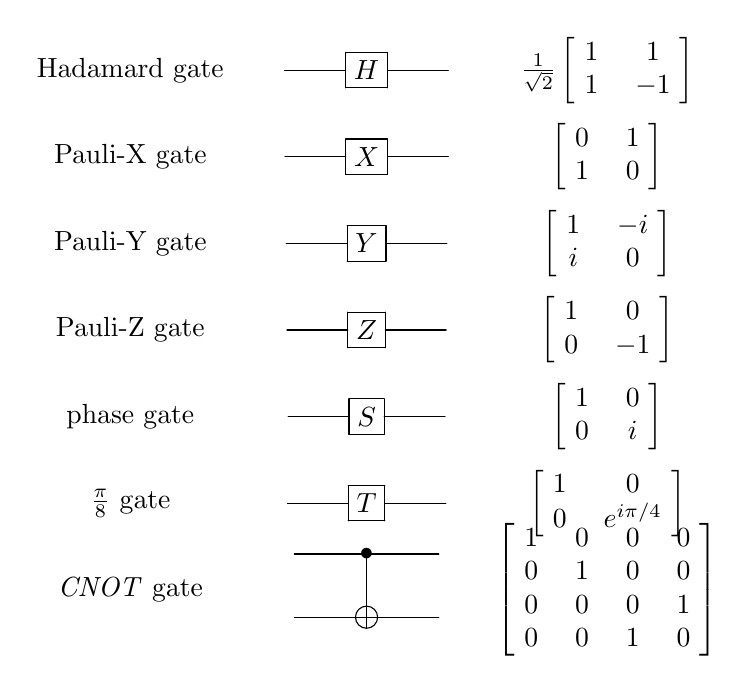
\begin{tikzpicture}
	% \textit{CNOT}
	\node at (7,0){	\textit{CNOT} gate };
	\node at (10,0){	
		\Qcircuit @C=2.2em @R=1.75em {
		 & \ctrl{1}  & \qw 	 \\
		 &\targ  	 & \qw   \\	    						 
	}};
	\node at (13,0){\vspace{10em}
				$\begin{bmatrix}
					\ 1\ & 0\ & 0\ & 0\ \\
					\ 0\ & 1\ & 0\ & 0\ \\
					\ 0\ & 0\ & 0\ & 1\ \\
					\ 0\ & 0\ & 1\ & 0\ 
				\end{bmatrix}$
	};

		% T
\node at (7,1.1){	$\frac{\pi}{8}$ gate };
\node at (10,1.1){	\Qcircuit @C=2.2em @R=1.75em {
	 & \gate{T}  & \qw 	 \\						 
}};
\node at (13,1.1){\vspace{10em}
			$\begin{bmatrix}
				\ 1\ & 0\  \\
				\ 0\ & e^{i\pi/4}\ \\
			\end{bmatrix}$
};
% phase gate
\node at (7,2.2){	phase gate };
\node at (10,2.2){	
	\Qcircuit @C=2.2em @R=1.75em {
	 & \gate{S}  & \qw 	 \\						 
}};
\node at (13,2.2){\vspace{10em}
			$\begin{bmatrix}
				\ 1\ & 0\  \\
				\ 0\ & i\ \\
			\end{bmatrix}$
};

% Z gate
\node at (7,3.3){	Pauli-Z gate };
\node at (10,3.3){	
	\Qcircuit @C=2.2em @R=1.75em {
	 & \gate{Z}  & \qw 	 \\						 
}};
\node at (13,3.3){\vspace{10em}
			$\begin{bmatrix}
				\ 1\ & 0\  \\
				\ 0\ & -1\ \\
			\end{bmatrix}$
};

% Y gate
\node at (7,4.4){	Pauli-Y gate };
\node at (10,4.4){	
	\Qcircuit @C=2.2em @R=1.75em {
	 & \gate{Y}  & \qw 	 \\						 
}};
\node at (13,4.4){\vspace{10em}
			$\begin{bmatrix}
				\ 1\ & -i\  \\
				\ i\ & 0\ \\
			\end{bmatrix}$
};
% X gate
\node at (7,5.5){	Pauli-X gate };
\node at (10,5.5){	
	\Qcircuit @C=2.2em @R=1.75em {
	 & \gate{X}  & \qw 	 \\						 
}};
\node at (13,5.5){\vspace{10em}
			$\begin{bmatrix}
				\ 0\ & 1\  \\
				\ 1\ & 0\ \\
			\end{bmatrix}$
};
% H
	% IBM Q20
	\node at (7,6.6){	Hadamard gate };
	\node at (10,6.6){	\Qcircuit @C=2.2em @R=1.75em {
		 & \gate{H}  & \qw 	 \\  						 
	}};
	\node at (13,6.6){\vspace{10em}
				$\frac{1}{\sqrt{2}}\begin{bmatrix}
					\ 1\ & 1\ \\
					\ 1\ & -1\ 
				\end{bmatrix}$
	};
\end{tikzpicture}
\end{center}

\caption{The symbols of common quantum gates and their matrices}\label{common_gates}
\end{figure}	 

}

\subsection{Quantum Circuit}
A quantum logical circuit $LC$ (see Fig.~\ref{OriginalCircuit})
consists of quantum gates interconnected by quantum wires~\cite{Daei2020}.
A quantum wire is a mechanism for moving quantum data from one location to another.
Each line represents a qubit, and the gates on the line act on the corresponding qubits.
The execution order of a quantum logical circuit graph is from left to right.
The width $w$ of a circuit refers to the number of qubits in the circuit.
The depth $d$ of a circuit refers to the number of layers executing in parallel.
For example, the depth of the circuit (see Fig.~\ref{OriginalCircuit}) is 6, and the width is 5.
In this paper, circuits with a depth less than 100 are called small-scale circuits,
circuits with a depth greater than 1000 are called large-scale circuits,
and the rest are medium-scale circuits.
It is unnecessary to consider single quantum gates in circuit transformation, since the single qubit is \emph{local}~\cite{2013Optimization}.


\begin{figure}[h!] 
	\begin{center}
		  {\scalefont{1.0}
	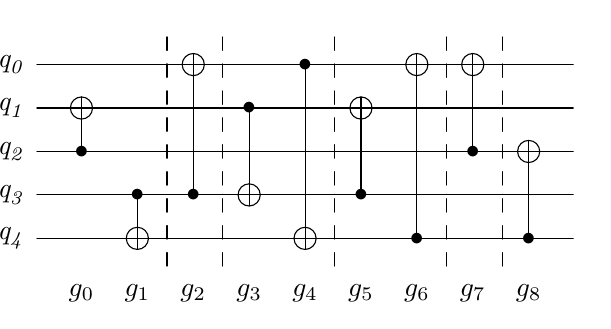
\begin{tikzpicture}
		% \draw[help lines] (0,0) grid (11,7);
		% IBM Q20
		\node at (5.5,5){  \Qcircuit @C=1.2em @R=0.75em {
			\lstick{\textit{q}_\textit{0}}   &  \qw 				&   \qw  \barrier{4}&\targ 	\barrier{4}	&\qw      		&\ctrl{4}\barrier{4}&   \qw		&\targ\barrier{4} &\targ  \barrier{4}&\qw  &  \qw       \\
			\lstick{\textit{q}_\textit{1}}   &   \targ      		&   \qw      		&   \qw      		&   \ctrl{2} 	&   \qw      	&   \targ    	&   \qw      	&   \qw       	&   \qw   		&  \qw       \\
			\lstick{\textit{q}_\textit{2}}   &   \ctrl{-1}  		&   \qw      		&   \qw      		&   \qw      	&   \qw      	&   \qw      	&   \qw     	&   \ctrl{-2} 	&   \targ       &  \qw       \\
			\lstick{\textit{q}_\textit{3}}   &\qw					&   \ctrl{1}   		&   \ctrl{-3} 		&   \targ    	&   \qw      	&   \ctrl{-2}	&   \qw      	&   \qw       	&   \qw        	&  \qw         \\
			\lstick{\textit{q}_\textit{4}}   &		\qw				& \targ				& \qw 				&   \qw      	&   \targ    	&   \qw      	&   \ctrl{-4}  	& 	\qw     	&   \ctrl{-2} 	&   \qw			\\
							  &\dstick{g_{0}}		&\dstick{g_{1}}		&\dstick{g_{2}}		&\dstick{g_{3}}	&\dstick{g_{4}} &\dstick{g_{5}} &\dstick{g_{6}} &\dstick{g_{7}} &\dstick{g_{8}}	&   		\\		 
							 &						&					&				&       		& 				& 				& 				&				&   				 
							 }};
	\end{tikzpicture}
	}
	\end{center}					 
	\caption{Original circuit}
	\label{OriginalCircuit}	
	 \end{figure}

	 \begin{figure}[h!] 
		\begin{center}
	{\scalefont{1}
		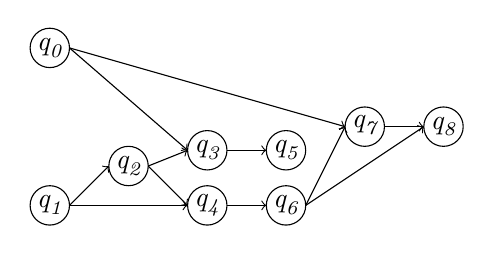
\begin{tikzpicture}							 
	\draw [black,  thin] (3,1) circle [radius=0.25];
	\draw [black,  thin] (3,3) circle [radius=0.25];
	\draw [black,  thin] (4,1.5) circle [radius=0.25];
	\draw [black,  thin] (5,1) circle [radius=0.25];
	\draw [black,  thin] (5,1.7) circle [radius=0.25];
	\draw [black,  thin] (6,1.7) circle [radius=0.25];
	\draw [black,  thin] (6,1) circle [radius=0.25];
	\draw [black,  thin] (7,2) circle [radius=0.25];
	\draw [black,  thin] (8,2) circle [radius=0.25];
	% label
	\node at (3,1) {$\textit{q}_\textit{1}$};
	\node at (3,3) {$\textit{q}_\textit{0}$};
	\node at (4,1.5) {$\textit{q}_\textit{2}$};
	\node at (5,1){$\textit{q}_\textit{4}$};
	\node at (5,1.7) {$\textit{q}_\textit{3}$};
	\node at (6,1.7){$\textit{q}_\textit{5}$};
	\node at (6,1) {$\textit{q}_\textit{6}$};
	\node at (7,2) {$\textit{q}_\textit{7}$};
	\node at (8,2) {$\textit{q}_\textit{8}$};

	% q1
	\draw [->, thin] (3.25,1) -- (3.75,1.5);
	\draw [->, thin] (3.25,1) -- (4.75,1);
	% q0
	\draw [->, thin] (3.25,3) -- (4.75,1.7);
	\draw [->, thin] (3.25,3) -- (6.75,2);
	% q2
	\draw [->, thin] (4.25,1.5) -- (4.75,1);
	\draw [->, thin] (4.25,1.5) -- (4.75,1.7);
	% q3
	\draw [->, thin] (5.25,1.7) -- (5.75,1.7);
	% q4
	\draw [->, thin] (5.25,1) -- (5.75,1);
	% q6
	\draw [->, thin] (6.25,1) -- (7.75,2);
	\draw [->, thin] (6.25,1) -- (6.75,2);
	% q7
	\draw [->, thin] (7.25,2) -- (7.75,2);
	\end{tikzpicture}
}
\end{center}
	\caption{The directed acyclic graph ($DAG$) of original circuit in Fig.~\ref{OriginalCircuit}}
	\label{DAG}
\end{figure}

\begin{figure}[h!]
	\begin{center}
		{\scalefont{1}
	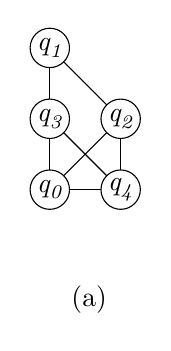
\begin{tikzpicture}
		% \tikzstyle{every node}=[font=\small,scale=0.9]

		\node at (0.5,0){(a)};
            % Q20
            \draw [black, thin] (0,1.4) circle [radius=0.25];
            \draw [-,thin] (0.25,1.4) -- (0.65,1.4);
            \draw [black, thin] (0.9,1.4) circle [radius=0.25];
            % label
            \node at (0,1.4) {$\textit{q}_\textit{0}$};
            \node at (0.9,1.4){$\textit{q}_\textit{4}$};
            % |
            \draw [-,thin] (0,1.65) -- (0,2.05);
            \draw [-,thin] (0.9,1.65)-- (0.9,2.05);
        
            \draw [black, thin] (0,2.3) circle [radius=0.25];
        
            \draw [black, thin] (0.9,2.3) circle [radius=0.25];
            % label
            \node at (0,2.3) {$\textit{q}_\textit{3}$};
            \node at (0.9,2.3){$\textit{q}_\textit{2}$};
            % |
            \draw [-,thin] (0,2.55) -- (0,2.95);
        
            \draw [black, thin] (0,3.2) circle [radius=0.25];
            \draw [-,thin] (0.175,3.025) -- (0.725,2.475);
            % label
            \node at (0,3.2) {$\textit{q}_\textit{1}$};
        
            %x
			\draw [-,thin] (0.175,2.125) -- (0.725,1.575);
			\draw [-,thin] (0.175,1.575) -- (0.725,2.125);
			\label{LLAG}
			\end{tikzpicture}
			}
			\qquad   \qquad
			{\scalefont{0.8}
			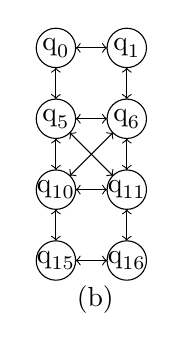
\begin{tikzpicture}
            
                % IBM Q20
            \node at (0.5,0){(b)};
            % Q20
            \draw [black, thin] (0,0.5) circle [radius=0.25];
            \draw [<->,thin] (0.25,0.5) -- (0.65,0.5);
            \draw [black, thin] (0.9,0.5) circle [radius=0.25];
        
            \node at (0,0.5) {$\textup{q}_\textup{15}$};
            \node at (0.9,0.5){$\textup{q}_\textup{16}$};
            % |
            \draw [<->,thin] (0,0.75) -- (0,1.15);
            \draw [<->,thin] (0.9,0.75) -- (0.9,1.15);
        
            \draw [black, thin] (0,1.4) circle [radius=0.25];
            \draw [<->,thin] (0.25,1.4) -- (0.65,1.4);
            \draw [black, thin] (0.9,1.4) circle [radius=0.25];
            % label
            \node at (0,1.4) {$\textup{q}_\textup{10}$};
            \node at (0.9,1.4){$\textup{q}_\textup{11}$};
            % |
            \draw [<->,thin] (0,1.65) -- (0,2.05);
            \draw [<->,thin] (0.9,1.65)-- (0.9,2.05);
        
            \draw [black, thin] (0,2.3) circle [radius=0.25];
            \draw [<->,thin] (0.25,2.3) -- (0.65,2.3);
            \draw [black, thin] (0.9,2.3) circle [radius=0.25];
            % label
            \node at (0,2.3) {$\textup{q}_\textup{5}$};
            \node at (0.9,2.3){$\textup{q}_\textup{6}$};
            % |
            \draw [<->,thin] (0,2.55) -- (0,2.95);
            \draw [<->,thin] (0.9,2.55)-- (0.9,2.95);
        
            \draw [black, thin] (0,3.2) circle [radius=0.25];
            \draw [<->,thin] (0.25,3.2) -- (0.65,3.2);
            \draw [black, thin] (0.9,3.2) circle [radius=0.25];
            % label
            \node at (0,3.2) {$\textup{q}_\textup{0}$};
            \node at (0.9,3.2){$\textup{q}_\textup{1}$};
        
            %x
        
            \draw [<->,thin] (0.175,2.125) -- (0.725,1.575);
			\draw [<->,thin] (0.175,1.575) -- (0.725,2.125);
			\label{PPAG}
	\end{tikzpicture}
			}
\end{center}
	
	\caption{(a) The architecture graph of original circuit in Fig.~\ref{OriginalCircuit}. (b) The partial architecture graph of IBM Q20.}
	\label{LAGPAG}
\end{figure}
	
\begin{figure}[h!] 			
	\centerline{ 
\Qcircuit @C=1.2em @R=0.5em {
							 &  \ctrl{2}  		&    \qw &   &    &  \gate{H}  		&\targ 			&\gate{H}     	&  \qw \\
							 &					&      	& 	\push{\rule{.3em}{0em}=\rule{.3em}{0em}}&	   &			& 				&	\\	 
							 &   \targ      	&    \qw 	&    &   &   \gate{H}      	&\ctrl{-2}      &\gate{H} 		&     \qw   \\	 
							&					&      	&		   &			&				& 				&					 
					}			
  }
  \centerline{ 
	\Qcircuit @C=1.2em @R=0.6em {
							\lstick{\textit{q}_\textit{0}} &  \qswap  				&    \rstick{\textit{q}_\textit{1}} \qw &&&&  \lstick{\textit{q}_\textit{0}} 	&  \ctrl{2}  		&  \targ  		&  \ctrl{2}  		&    \rstick{\textit{q}_\textit{1}} \qw &&&&  \lstick{\textit{q}_\textit{0}}  &  \ctrl{2}  		&   \gate{H}  		&\ctrl{2} 			&\gate{H}     	&\ctrl{2}			&    \rstick{\textit{q}_\textit{1}}\qw  \\
							&		\qwx	&&&\push{\rule{.3em}{0em}=\rule{.3em}{0em}}&		&  	&					&			
							&		&      	& 		&	\push{\rule{.3em}{0em}=\rule{.3em}{0em}}					&					&				&					&         			&&&&			 \\
							\lstick{\textit{q}_\textit{1}} &   \qswap\qwx	   		&     \rstick{\textit{q}_\textit{0}}  \qw &&&&    \lstick{\textit{q}_\textit{1}} 	&   \targ      		&  \ctrl{-2}    &   \targ      		&     \rstick{\textit{q}_\textit{0}}  \qw   &&&&  \lstick{\textit{q}_\textit{1}}  &   \targ      		&   \gate{H}      	&   \targ      		&\gate{H} 		&\targ      		&    \rstick{\textit{q}_\textit{0}}\qw 	   \\	 
																	&			&&&&		&  	&					&					&					&       		& 					&						&					&				&					&         			&&&&			 
						} 
}
						\caption{The above circuit changes the direction of the \textit{CNOT} gate by adding four H gates, and  below is the circuit of the \textit{SWAP} gate.}
						\label{Decomposition}
\end{figure}

\subsection{Architectures}
We mainly discuss the physical circuits of IBM Q series.
Let $\mathcal{\mathcal{AG}_{P}}=(V_{P}, E_{P})$ denote the architecture graph of the physical circuit,
where $V_{P}$ denotes the physical qubit set and $E_{P}$ denotes the edge set that the \textit{CNOT} gates.
Fig.~\ref{IBM} (a) and (b) are \textit{PAG} of the 5-qubit of IBM QX2,
(c) and (d) are \textit{PAG} of 16-qubit of IBM QX3,
and (e) is the \textit{PAG} of IBM Q20.
The arrow direction in the figure indicates the control direction of the gate,
and the 2-qubit gate can only be performed between qubits with edges connected.
IBM physical circuits only support single quantum gates and \textit{CNOT} gates between two adjacent qubits.

Given a logical circuit $LC$, a physical structure $\mathcal{AG}_{P}$, an initial mapping $\tau$, and a \textit{CNOT} gate $g=\left \langle \textit{q}_\textit{i},\textit{q}_\textit{j}\right \rangle $, where $\textit{q}_\textit{i}$ is the control qubit, $\textit{q}_\textit{j}$ is the target qubit.
$\left \langle\tau(\textit{q}_\textit{i}),\tau(\textit{q}_\textit{j})\right \rangle $ 
is a directed edge on $\mathcal{AG}_{P}$, if gate $g$ is executable.

\begin{example}
	Fig.~\ref{LAGPAG} (a) is the logical structure of Fig.~\ref{OriginalCircuit}, 
	Fig.~\ref{LAGPAG} (b) is the partial architecture graph of IBM Q20, the initial mapping is 
	$\tau=\{\textit{q}_\textit{0}\rightarrow  \textup{q}_{\textup{10}},\ \textit{q}_\textit{1}\rightarrow \textup{q}_{\textup{0}},\ 
	\textit{q}_\textit{2}\rightarrow  \textup{q}_{\textup{6}},\ \textit{q}_\textit{3}\rightarrow  \textup{q}_{\textup{5}},\ \textit{q}_\textit{4}\rightarrow  \textup{q}_{\textup{11}}\}$.
	$g_{0}=\left \langle \textit{q}_\textit{2},\textit{q}_\textit{1}\right \rangle $ is not executable, since the edge $\left \langle \tau(\textit{q}_\textit{2}),\tau(\textit{q}_\textit{1})\right \rangle =\left \langle \textup{q}_{\textup{6}},\textup{q}_{\textup{0}}\right \rangle $ does not exist in $\mathcal{AG}_{P}$.
	But $g_{3}=\left \langle \textit{q}_\textit{1},\textit{q}_\textit{3}\right \rangle $ is executable, since 
	the edge $\left \langle \tau(\textit{q}_\textit{1}),\tau(\textit{q}_\textit{3})\right \rangle =\left \langle \textup{q}_{\textup{0}},\textup{q}_{\textup{5}}\right \rangle $  exist in $\mathcal{AG}_{P}$.
\end{example}
\begin{figure}
	{
	\scalefont{0.8}
	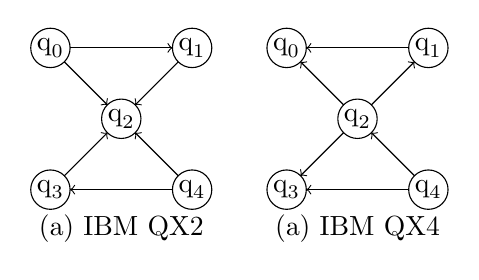
\begin{tikzpicture}
	% \draw[help lines] (0,0) grid (11,3);
		% IBM QX2
	\node at (1.8,0.4){(a) IBM QX2};
	\node at (4.8,0.4){(a) IBM QX4};
	% label
	\node at (0.9,2.7){$\textup{q}_\textup{0}$};
	\draw [black, thin] (0.9,2.7) circle [radius=0.25];
	\node at (2.7,2.7){$\textup{q}_\textup{1}$};
	\draw [black, thin] (2.7,2.7) circle [radius=0.25];
	\node at (1.8,1.8){$\textup{q}_\textup{2}$};
	\draw [black, thin] (1.8,1.8)circle [radius=0.25];
	\node at (0.9,0.9){$\textup{q}_\textup{3}$};
	\draw [black, thin] (0.9,0.9) circle [radius=0.25];
	\node at (2.7,0.9){$\textup{q}_\textup{4}$};
	\draw [black, thin] (2.7,0.9) circle [radius=0.25];

	
	% -
	\draw [->,thin] (1.15,2.7) -- (2.45,2.7);
	
	\draw [<-,thin] (1.15,0.9) -- (2.45,0.9);

	%x
	\draw [->,thin] (1.075,2.525) -- (1.625,1.975);
	\draw [->,thin] (2.525,2.525) -- (1.975,1.975);
	\draw [->,thin] (1.075,1.075) -- (1.625,1.625);
	\draw [->,thin] (2.525,1.075) -- (1.975,1.625);

		 
		% label
		\node at (3.9,2.7){$\textup{q}_\textup{0}$};
		\draw [black, thin] (3.9,2.7) circle [radius=0.25];
		\node at (5.7,2.7){$\textup{q}_\textup{1}$};
		\draw [black, thin] (5.7,2.7) circle [radius=0.25];
		\node at (4.8,1.8){$\textup{q}_\textup{2}$};
		\draw [black, thin] (4.8,1.8)circle [radius=0.25];
		\node at (3.9,0.9){$\textup{q}_\textup{3}$};
		\draw [black, thin] (3.9,0.9) circle [radius=0.25];
		\node at (5.7,0.9){$\textup{q}_\textup{4}$};
		\draw [black, thin] (5.7,0.9) circle [radius=0.25];
		
		% -
		\draw [<-,thin] (4.15,2.7) -- (5.45,2.7);
		
		\draw [<-,thin] (4.15,0.9) -- (5.45,0.9);

		\draw [<-,thin] (4.075,2.525) -- (4.625,1.975);
		\draw [<-,thin] (5.525,2.525) -- (4.975,1.975);
		\draw [<-,thin] (4.075,1.075) -- (4.625,1.625);
		\draw [->,thin] (5.525,1.075) -- (4.975,1.625);
	
	\end{tikzpicture}
}
\\
{
	\scalefont{0.8}
		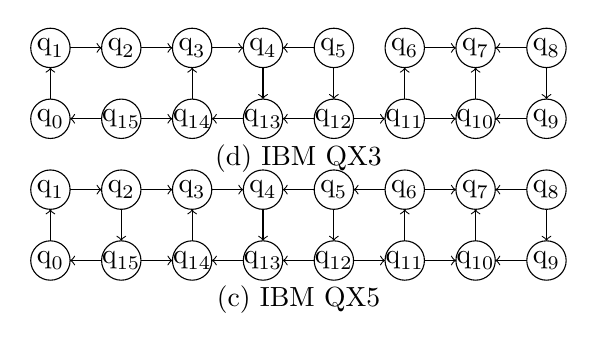
\begin{tikzpicture}
			
	\node at (3.15,0){(c) IBM QX5};
	\node at (3.15,1.8){(d) IBM QX3};
		%QX5
		%-
	\draw [black, thin] (0,2.3) circle [radius=0.25];
	\draw [<-,thin] (0.25,2.3) -- (0.65,2.3);
	\draw [black, thin] (0.9,2.3) circle [radius=0.25];
	\draw [->,thin] (1.15,2.3) -- (1.55,2.3);
	\draw [black, thin] (1.8,2.3) circle [radius=0.25];
	\draw [<-,thin] (2.05,2.3) -- (2.45,2.3);
	\draw [black, thin] (2.7,2.3) circle [radius=0.25];
	\draw [<-,thin] (2.95,2.3) -- (3.35,2.3);
	\draw [black, thin] (3.6,2.3) circle [radius=0.25];
	\draw [->,thin] (3.85,2.3) -- (4.25,2.3);
	\draw [black, thin] (4.5,2.3) circle [radius=0.25];
	\draw [->,thin] (4.75,2.3) -- (5.15,2.3);
	\draw [black, thin] (5.4,2.3) circle [radius=0.25];
	\draw [<-,thin] (5.65,2.3) -- (6.05,2.3);
	\draw [black, thin] (6.3,2.3) circle [radius=0.25];

	% |
	\draw [->,thin] (0,2.55) -- (0,2.95);
	\draw [->,thin] (1.8,2.55) -- (1.8,2.95);
	\draw [<-,thin] (2.7,2.55) -- (2.7,2.95);
	\draw [<-,thin] (3.6,2.55) -- (3.6,2.95);
	\draw [->,thin] (4.5,2.55) -- (4.5,2.95);
	\draw [->,thin] (5.4,2.55) -- (5.4,2.95);
	\draw [<-,thin] (6.3,2.55) -- (6.3,2.95);
	%-
\draw [black, thin] (0,3.2) circle [radius=0.25];
\draw [->,thin] (0.25,3.2) -- (0.65,3.2);
\draw [black, thin] (0.9,3.2) circle [radius=0.25];
\draw [->,thin] (1.15,3.2) -- (1.55,3.2);
\draw [black, thin] (1.8,3.2) circle [radius=0.25];
\draw [->,thin] (2.05,3.2) -- (2.45,3.2);
\draw [black, thin] (2.7,3.2) circle [radius=0.25];
\draw [<-,thin] (2.95,3.2) -- (3.35,3.2);
\draw [black, thin] (3.6,3.2) circle [radius=0.25];

\draw [black, thin] (4.5,3.2) circle [radius=0.25];
\draw [->,thin] (4.75,3.2) -- (5.15,3.2);
\draw [black, thin] (5.4,3.2) circle [radius=0.25];
\draw [<-,thin] (5.65,3.2) -- (6.05,3.2);
\draw [black, thin] (6.3,3.2) circle [radius=0.25];
	
	% label
	\node at (0,0.5){$\textup{q}_\textup{0}$};
	\node at (0.9,0.5){$\textup{q}_\textup{15}$};
	\node at (1.8,0.5){$\textup{q}_\textup{14}$};
	\node at (2.7,0.5){$\textup{q}_\textup{13}$};
	\node at (3.6,0.5){$\textup{q}_\textup{12}$};
	\node at (4.5,0.5){$\textup{q}_\textup{11}$};
	\node at (5.4,0.5){$\textup{q}_\textup{10}$};
	\node at (6.3,0.5){$\textup{q}_\textup{9}$};

	\node at (0,1.4){$\textup{q}_\textup{1}$};
	\node at (0.9,1.4){$\textup{q}_\textup{2}$};
	\node at (1.8,1.4){$\textup{q}_\textup{3}$};
	\node at (2.7,1.4){$\textup{q}_\textup{4}$};
	\node at (3.6,1.4){$\textup{q}_\textup{5}$};
	\node at (4.5,1.4){$\textup{q}_\textup{6}$};
	\node at (5.4,1.4){$\textup{q}_\textup{7}$};
	\node at (6.3,1.4){$\textup{q}_\textup{8}$};

		%QX5
		%-
		\draw [black, thin] (0,0.5) circle [radius=0.25];
		\draw [<-,thin] (0.25,0.5) -- (0.65,0.5);
		\draw [black, thin] (0.9,0.5) circle [radius=0.25];
		\draw [->,thin] (1.15,0.5) -- (1.55,0.5);
		\draw [black, thin] (1.8,0.5) circle [radius=0.25];
		\draw [<-,thin] (2.05,0.5) -- (2.45,0.5);
		\draw [black, thin] (2.7,0.5) circle [radius=0.25];
		\draw [<-,thin] (2.95,0.5) -- (3.35,0.5);
		\draw [black, thin] (3.6,0.5) circle [radius=0.25];
		\draw [->,thin] (3.85,0.5) -- (4.25,0.5);
		\draw [black, thin] (4.5,0.5) circle [radius=0.25];
		\draw [->,thin] (4.75,0.5) -- (5.15,0.5);
		\draw [black, thin] (5.4,0.5) circle [radius=0.25];
		\draw [<-,thin] (5.65,0.5) -- (6.05,0.5);
		\draw [black, thin] (6.3,0.5) circle [radius=0.25];
	
		% |
		\draw [->,thin] (0,0.75) -- (0,1.15);
		\draw [<-,thin] (0.9,0.75) -- (0.9,1.15);
		\draw [->,thin] (1.8,0.75) -- (1.8,1.15);
		\draw [<-,thin] (2.7,0.75) -- (2.7,1.15);
		\draw [<-,thin] (3.6,0.75) -- (3.6,1.15);
		\draw [->,thin] (4.5,0.75) -- (4.5,1.15);
		\draw [->,thin] (5.4,0.75) -- (5.4,1.15);
		\draw [<-,thin] (6.3,0.75) -- (6.3,1.15);
		%-
	\draw [black, thin] (0,1.4) circle [radius=0.25];
	\draw [->,thin] (0.25,1.4) -- (0.65,1.4);
	\draw [black, thin] (0.9,1.4) circle [radius=0.25];
	\draw [->,thin] (1.15,1.4) -- (1.55,1.4);
	\draw [black, thin] (1.8,1.4) circle [radius=0.25];
	\draw [->,thin] (2.05,1.4) -- (2.45,1.4);
	\draw [black, thin] (2.7,1.4) circle [radius=0.25];
	\draw [<-,thin] (2.95,1.4) -- (3.35,1.4);
	\draw [black, thin] (3.6,1.4) circle [radius=0.25];
	\draw [<-,thin] (3.85,1.4) -- (4.25,1.4);
	\draw [black, thin] (4.5,1.4) circle [radius=0.25];
	\draw [->,thin] (4.75,1.4) -- (5.15,1.4);
	\draw [black, thin] (5.4,1.4) circle [radius=0.25];
	\draw [<-,thin] (5.65,1.4) -- (6.05,1.4);
	\draw [black, thin] (6.3,1.4) circle [radius=0.25];
		
		% label
		\node at (0,2.3){$\textup{q}_\textup{0}$};
		\node at (0.9,2.3){$\textup{q}_\textup{15}$};
		\node at (1.8,2.3){$\textup{q}_\textup{14}$};
		\node at (2.7,2.3){$\textup{q}_\textup{13}$};
		\node at (3.6,2.3){$\textup{q}_\textup{12}$};
		\node at (4.5,2.3){$\textup{q}_\textup{11}$};
		\node at (5.4,2.3){$\textup{q}_\textup{10}$};
		\node at (6.3,2.3){$\textup{q}_\textup{9}$};
	
		\node at (0,3.2){$\textup{q}_\textup{1}$};
		\node at (0.9,3.2){$\textup{q}_\textup{2}$};
		\node at (1.8,3.2){$\textup{q}_\textup{3}$};
		\node at (2.7,3.2){$\textup{q}_\textup{4}$};
		\node at (3.6,3.2){$\textup{q}_\textup{5}$};
		\node at (4.5,3.2){$\textup{q}_\textup{6}$};
		\node at (5.4,3.2){$\textup{q}_\textup{7}$};
		\node at (6.3,3.2){$\textup{q}_\textup{8}$};
	\end{tikzpicture}
}
{\scalefont{0.8}
	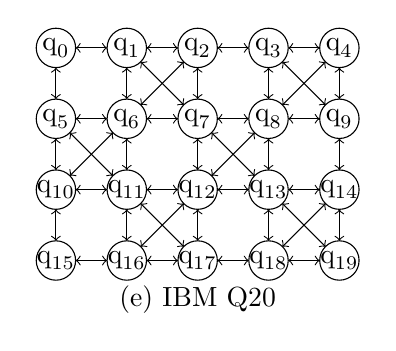
\begin{tikzpicture}
	
		% IBM Q20
		\node at (1.8,0){(e) IBM Q20};
	% Q20
	\draw [black, thin] (0,0.5) circle [radius=0.25];
	\draw [<->,thin] (0.25,0.5) -- (0.65,0.5);
	\draw [black, thin] (0.9,0.5) circle [radius=0.25];
	\draw [<->,thin] (1.15,0.5) -- (1.55,0.5);
	\draw [black, thin] (1.8,0.5) circle [radius=0.25];
	\draw [<->,thin] (2.05,0.5) -- (2.45,0.5);
	\draw [black, thin] (2.7,0.5) circle [radius=0.25];
	\draw [<->,thin] (2.95,0.5) -- (3.35,0.5);
	\draw [black, thin] (3.6,0.5) circle [radius=0.25];

	\node at (0,0.5) {$\textup{q}_\textup{15}$};
	\node at (0.9,0.5){$\textup{q}_\textup{16}$};
	\node at (1.8,0.5){$\textup{q}_\textup{17}$};
	\node at (2.7,0.5){$\textup{q}_\textup{18}$};
	\node at (3.6,0.5){$\textup{q}_\textup{19}$};
	% |
	\draw [<->,thin] (0,0.75) -- (0,1.15);
	\draw [<->,thin] (0.9,0.75) -- (0.9,1.15);
	\draw [<->,thin] (1.8,0.75) -- (1.8,1.15);
	\draw [<->,thin] (2.7,0.75) -- (2.7,1.15);
	\draw [<->,thin] (3.6,0.75) -- (3.6,1.15);

	\draw [black, thin] (0,1.4) circle [radius=0.25];
	\draw [<->,thin] (0.25,1.4) -- (0.65,1.4);
	\draw [black, thin] (0.9,1.4) circle [radius=0.25];
	\draw [<->,thin] (1.15,1.4) -- (1.55,1.4);
	\draw [black, thin] (1.8,1.4)circle [radius=0.25];
	\draw [<->,thin] (2.05,1.4) -- (2.45,1.4);
	\draw [black, thin] (2.7,1.4) circle [radius=0.25];
	\draw [<->,thin] (2.95,1.4) -- (3.35,1.4);
	\draw [black, thin] (3.6,1.4) circle [radius=0.25];
	% label
	\node at (0,1.4) {$\textup{q}_\textup{10}$};
	\node at (0.9,1.4){$\textup{q}_\textup{11}$};
	\node at (1.8,1.4){$\textup{q}_\textup{12}$};
	\node at (2.7,1.4){$\textup{q}_\textup{13}$};
	\node at (3.6,1.4){$\textup{q}_\textup{14}$};
	% |
	\draw [<->,thin] (0,1.65) -- (0,2.05);
	\draw [<->,thin] (0.9,1.65)-- (0.9,2.05);
	\draw [<->,thin] (1.8,1.65) -- (1.8,2.05);
	\draw [<->,thin] (2.7,1.65) -- (2.7,2.05);
	\draw [<->,thin] (3.6,1.65) -- (3.6,2.05);

	\draw [black, thin] (0,2.3) circle [radius=0.25];
	\draw [<->,thin] (0.25,2.3) -- (0.65,2.3);
	\draw [black, thin] (0.9,2.3) circle [radius=0.25];
	\draw [<->,thin] (1.15,2.3) -- (1.55,2.3);
	\draw [black, thin] (1.8,2.3)circle [radius=0.25];
	\draw [<->,thin] (2.05,2.3) -- (2.45,2.3);
	\draw [black, thin] (2.7,2.3) circle [radius=0.25];
	\draw [<->,thin] (2.95,2.3) -- (3.35,2.3);
	\draw [black, thin] (3.6,2.3) circle [radius=0.25];
	% label
	\node at (0,2.3) {$\textup{q}_\textup{5}$};
	\node at (0.9,2.3){$\textup{q}_\textup{6}$};
	\node at (1.8,2.3){$\textup{q}_\textup{7}$};
	\node at (2.7,2.3){$\textup{q}_\textup{8}$};
	\node at (3.6,2.3){$\textup{q}_\textup{9}$};
	% |
	\draw [<->,thin] (0,2.55) -- (0,2.95);
	\draw [<->,thin] (0.9,2.55)-- (0.9,2.95);
	\draw [<->,thin] (1.8,2.55) -- (1.8,2.95);
	\draw [<->,thin] (2.7,2.55) -- (2.7,2.95);
	\draw [<->,thin] (3.6,2.55) -- (3.6,2.95);

	\draw [black, thin] (0,3.2) circle [radius=0.25];
	\draw [<->,thin] (0.25,3.2) -- (0.65,3.2);
	\draw [black, thin] (0.9,3.2) circle [radius=0.25];
	\draw [<->,thin] (1.15,3.2) -- (1.55,3.2);
	\draw [black, thin] (1.8,3.2)circle [radius=0.25];
	\draw [<->,thin] (2.05,3.2) -- (2.45,3.2);
	\draw [black, thin] (2.7,3.2) circle [radius=0.25];
	\draw [<->,thin] (2.95,3.2) -- (3.35,3.2);
	\draw [black, thin] (3.6,3.2) circle [radius=0.25];
	% label
	\node at (0,3.2) {$\textup{q}_\textup{0}$};
	\node at (0.9,3.2){$\textup{q}_\textup{1}$};
	\node at (1.8,3.2){$\textup{q}_\textup{2}$};
	\node at (2.7,3.2){$\textup{q}_\textup{3}$};
	\node at (3.6,3.2){$\textup{q}_\textup{4}$};

	%x
	\draw [<->,thin] (1.075,0.675) -- (1.625,1.225);
	\draw [<->,thin] (1.075,1.225) -- (1.625,0.675);
	\draw [<->,thin] (2.875,0.675) -- (3.425,1.225);
	\draw [<->,thin] (2.875,1.225) -- (3.425,0.675);
		%3
	\draw [<->,thin] (1.075,2.475) -- (1.625,3.025);
	\draw [<->,thin] (1.075,3.025) -- (1.625,2.475);
	\draw [<->,thin] (2.875,2.475) -- (3.425,3.025);
	\draw [<->,thin] (2.875,3.025) -- (3.425,2.475);
		% 2
	\draw [<->,thin] (0.175,2.125) -- (0.725,1.575);
	\draw [<->,thin] (0.175,1.575) -- (0.725,2.125);
	\draw [<->,thin] (1.975,2.125) -- (2.525,1.575);
	\draw [<->,thin] (1.975,1.575) -- (2.525,2.125);
	\end{tikzpicture}
}
\caption{IBM QX architectures}
\label{IBM}
\end{figure}


\section{Problem Analysis}
\label{Problem Analysis}
Single qubit gates and \textit{CNOT} gates are used as basic gates, since they are commonly used to implement any quantum circuit supported by the IBM QX architecture. Before circuit transformation, the circuit should be simplified to a circuit with only single quantum gates and \textit{CNOT} gates~\cite{2005Mttnen,1995Barenco}. We insert auxiliary gates (see Fig.~\ref{Decomposition}) to move two non-adjacent quantum positions to adjacent positions or change the direction of the \textit{CNOT} gate, but this process may introduce errors. The introduction of auxiliary gates may lead to errors. We hope to find a circuit transformation algorithm to make the output circuit with the minimum number of auxiliary gates and the circuit depth in an acceptable amount of time.
A quantum circuit transformation problem mainly includes the following four steps. Isomorphism and transformation are both NPCs~\cite{2018QubitSiraichi}.
\begin{figure}[h!] 
	\centering
	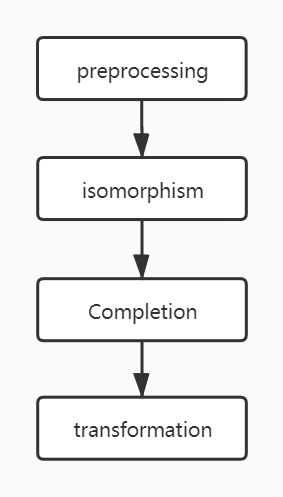
\includegraphics[scale=0.4]{uml.jpg}		 
	\caption{Circuit transformation process}
	\label{processing}	
	 \end{figure}
\begin{enumerate}
	\item \emph{ Preprocess the logical quantum circuit.} 
	It includes extracting the logical architecture graph (\textit{LAG}) of the circuit, adjusting the life cycle of qubits (the work is done by Zhang~\cite{2019Zhang}),  and calculating the shortest paths of the physical circuit.
	\item \emph{Compute isomorphic substructures.}
	It uses the subgraph isomorphism algorithm to find part of the initial mapping, which is done by Sun~\cite{Sun2020}.
	\item \emph{Generate a high-quality initial mapping.} We perform mapping completion because the remaining nodes cannot satisfy all isomorphism requirements. According to the connectivity between the unmapped node and the mapped nodes. Unmapped nodes are mapped to the neighborhood of mapped nodes, which satisfies the connectivity of part of the \textit{LAG} and \textit{PAG} and reduces the length of the shortest path.  
	\item \emph{Transforming logical circuits to meet physical constraints.}
	Circuit transformation need to be solved before quantum circuits compilation, since he design of quantum algorithms does not refer to the connectivity constraints of any hardware. Therefore, It is necessary for any quantum compiler.
\end{enumerate}

\section{Solution}
\label{Solution}
The solution proposed in this paper mainly includes preprocessing, initial mapping, and circuit transformation. In this section, we will introduce them in detail.
\subsection{Preprocessing}
Before circuit transformation, we can preprocess it to get more convenient data to shorten our search time and space. In the preprocessing, we adjust the circuit of the input openQASM program to shorten the life cycle of qubits. Then we use Breadth-First Search (\textit{BFS}) to calculate the shortest distance between each node on the architecture graph.
\subsubsection{Circuit Adjustment}
We use a layered method to analyze the life cycle of qubits and pack the gates that can be executed in parallel into a $bundle$, forming a layered bundle format~\cite{2019Zhang}.
A conversion method is designed to use the layered bundle format to determine which gates can be moved, which reduces the life cycle of these qubits. The algorithm reduces the error rate of quantum programs by 11\%. In most quantum workloads, the longest qubit lifetime and the average qubit lifetime can be reduced by more than 20\%, and the execution time of some quantum programs can also be reduced.
\subsubsection{Shortest Distance}
Given \textit{PAG} and the distance of each edge is 1, we can use \textit{Floyd-Warshall} algorithm calculate the shortest distance matrix $dist[i][j]$, which represents the shortest distance from $\textup{q}_{\textup{i}}$ to $\textup{q}_{\textup{j}}$. 

For IBM QX2, QX3, QX4, QX5, a \textit{SWAP} needs 7 gates (3 \textit{CNOT} gates and 4 $H$ gates). Only 4 $H$ gates are needed to change the direction of an adjacent \textit{CNOT} gate. 
For a \textit{CNOT} gate $g=\left \langle  \textit{q}_\textit{i},\textit{q}_\textit{j} \right \rangle $,
two qubits are mapped to $\textup{q}_{m}$ and $\textup{q}_{n}$, respectively, with $\tau(\textit{q}_\textit{i})=\textup{q}_{\textup{m}},\tau(\textit{q}_\textit{j})=\textup{q}_{\textup{n}}$. Then the cost of executing $g$ under the shortest distance path is $cost_{cnot}(\textit{q}_\textit{i},\textit{q}_\textit{j})=7 \times( dist[m][n]-1)$. For IBM Q20, in which all edges are bidirectional, a \textit{SWAP} requires 3 \textit{CNOT} gates. Thus the cost between them is $cost_{cnot}(\textit{q}_\textit{i},\textit{q}_\textit{j})=3 \times( dist[m][n]-1)$. The time complexity is $O (N^{3})$.
\begin{example}
	Take the QX5 structure as an example. Suppose there is a \textit{CNOT} gate $g=\left \langle  \textit{q}_\textit{i}, \textit{q}_\textit{j} \right \rangle $, \ $\textit{q}_\textit{i}$ is mapped to $\textup{q}_{1}$,  $\textit{q}_\textit{j}$ is mapped to $\textup{q}_{\textup{14}}$, and the shortest distance between them  is $dist[1][14]=3$. There are 3 shortest paths to move $\textup{q}_{\textup{1}}$ to the adjacent position of 
$\textup{q}_{\textup{14}}$:
$\Pi=\{\pi_{0},\pi_{1},\pi_{2}\}$, 
$\pi_{0}={\textup{q}_{\textup{1}}\rightarrow \textup{q}_{\textup{2}} \rightarrow \textup{q}_{\textup{3}} \rightarrow \textup{q}_{\textup{14}}}$,
$\pi_{1}={\textup{q}_{\textup{1}}\rightarrow \textup{q}_{\textup{2}} \rightarrow \textup{q}_{\textup{15}} \rightarrow \textup{q}_{\textup{14}}}$,
$\pi_{2}={\textup{q}_{\textup{1}}\rightarrow \textup{q}_{\textup{0}} \rightarrow \textup{q}_{\textup{15}} \rightarrow \textup{q}_{\textup{14}}}$.
Their costs are 
$cost_{\pi_{0}}=18,\ cost_{\pi_{1}}=14,\ cost_{\pi_{2}}=14$, respectively.
\end{example}

\subsubsection{Circuit Layering}
Quantum gates acting on different qubits can execute in parallel. Therefore, we classify the gates that can be executed in parallel into one layer, otherwise add a new layer. $L(LC)=\{\mathcal{L}_{0},\mathcal{L}_{1},...,\mathcal{L}_{n}\}$ represents the layered circuit, where $\mathcal{L}_{i} \ (0 \le i \le n) $ represents a quantum gate set that can be executed in parallel. The quantum gate set separated by the dotted line in Fig.~\ref{OriginalCircuit} are the following $\mathcal{L}_{0}=\{g_{0},g_{1}\},\mathcal{L}_{1}=\{g_{2}\},
 \mathcal{L}_{2}=\{g_{3},g_{4}\},\mathcal{L}_{3}=\{g_{5},g_{6}\},\mathcal{L}_{4}=\{g_{7}\},\mathcal{L}_{5}=\{g_{8}\}$.

At the same time, we generate logical circuit architecture graph $\mathcal{AG_{L}}=(V_{L},E_{L})$, which is an undirected graph. $V_{L}$ contains the vertices and the degree of each vertex, and $E_{L}$ represents the set of undirected edges that the \textit{CNOT} gates can execute.

\subsection{Initial Mapping}
It has been proved that the initial mapping has an important  influence on quantum circuit transformation,  and the subgraph isomorphism can be reduced to initial mapping problem. Thus we use the subgraph isomorphism algorithm to find a partial initial mapping that helps to minimize auxiliary gates added by the output circuit.

In \textit{PAG}, it is almost impossible to find a subgraph that exactly matched nodes \textit{LAG}. Thus we regard the mapping with the largest number of matching nodes as the partial mapping. \textit{SubgraphCompare}~\cite{Sun2020} compares several state-of-the-art subgraph isomorphism algorithm composition. 
It shows that using the filtering and sorting ideas of \emph{GraphQL} algorithm to process candidate nodes, and the local candidates calculation method \emph{LFTJ} based on set-intersection to enumerate the results is the best. We artificially connect the isolating qubits to the qubits with the largest degree in the logical architecture graph, since \textit{SubgraphCompare} cannot handle the not connected graph. We want to minimize the impact of logical dependency graph, so match it with the node with the largest degree.

\begin{algorithm}  
	\label{algorithm_initial}
	\caption{initial mapping algorithm \textit{CSI}}  
	\LinesNumbered  
	\KwIn{$\mathcal{AG_{L}}$: The architecture of logical circuit \\ 
	$\mathcal{AG_{P}}$: The architecture of physical circuit\\
	$T$: A partial mapping set obtained by \textit{SubgraphCompare}  \\
	}
	\KwOut{$result$: A collection of mapping relations between
	 $\mathcal{AG_{L}}$ and $\mathcal{AG_{P}}$}  
	\textbf{Initialize} $result=\emptyset$ ;\\
	$l \leftarrow max_{\tau \in T} \  \tau.length$; \\
	\For{$\tau\in T$}{
		\If{$l=\tau.length$}{
			$result.add(\tau)$;\\
			$Q \leftarrow $ initialing an empty unmapped node queue \\
			$i \leftarrow  1$; \\ 
			\While{$i\leq \tau.length$}{
				\If{$\tau[i]=-1$}{
					$Q \leftarrow {i}$;
				}
				$i \leftarrow i+1$;
			}
			\While{$Q\ is\ not\ empty$}{
				int  $\textit{q} \leftarrow Q.poll()$;\\
				$targetAdj \leftarrow$ $\mathcal{AG_{P}}.adjacencyMatrix()$; 	\\
				$queryAdj \leftarrow$ $\mathcal{AG_{L}}.adjacencyMatrix()$;	\\
				$cans \leftarrow$ initialing an empty candidate node list \tcp*{sorted by the connectivity of nodes }
				\ForEach{$\textit{q}_\textit{m} \leq queryAdj[\textit{q}].length$}{
					$cans \leftarrow cans \cup \{ \textit{q}_\textit{m}\}$;	
				}
				\While{$cans\ is\ not\ empty$}{
					$\textup{q} \leftarrow \tau[cans.first]$; \\
					$k \leftarrow 0$; \\
					$cans \leftarrow cans\backslash cans.first$; \\
					\While{$ k \textless targetAdj[\textup{q}].length$}{
						\If{  $(targetAdj[\textup{q}][k]\neq -1\ or\ targetAdj[k][\textup{q}]  \neq -1)$\\
						  $\ and\ not\ \tau.contains(k)$}{
							 $\tau[\textit{q}] \leftarrow k$; \\
							 break;
						 }
						  $k \leftarrow k+1$;
					}
					\If{ $k\neq targetAdj[\textup{q}].length$ }{
						break;
					}
				}
			}
		}
	}
	\end{algorithm}
	
	The input of Algorithm~\ref{algorithm_initial} is a target graph ($\mathcal{AG}_{P}$), a query graph ($\mathcal{AG}_{L}$), and the partial mappings $T$. First, we initialize an empty queue $Q$.
	Then we traverse $\tau$ and add the unmapped nodes to the queue $Q$. For the unmapped nodes, we try to map them to the vicinity of the mapped nodes in $\mathcal{AG}_{P}$. Finally, generate a dense mapping, which can reduce the added auxiliary gates. We would try to match the remaining unmapped nodes randomly, but it may lead to mapping to a node far away from other nodes. If the unmapped node has an edge adjacent to the matched point in the query graph, it will be matched to one of the adjacent nodes first.  Finally, we get all initial candidate mappings.

	In Algorithm~\ref{algorithm_initial}, lines 2 selects the partial mapping with the most mapped nodes $l$ as the candidate set. Lines 3-41 completes the logical qubit unmapped nodes in the candidate set. In line 6, we initialized an empty queue $Q$, which stores unmapped logical qubits. In lines 8-13, we traverse the mapping $\tau$ and add the unmapped qubits to $Q$. We loop until $Q$ is empty, and all logical qubits map to physical qubits. We take out the first element in $Q$ to \textit{q}. Lines 16 and 17 are used to get the adjacency matrices of $\mathcal{AG}_{P}$ and $\mathcal{AG}_{L}$, respectively. Line 18 initializes an empty map $cans$, sort by descending order of whether $\textit{q}_\textit{m}$ is mapped and the number of gate appearances. Lines 20-22 store the nodes $\textit{q}_\textit{m}$ connected to \textit{q} in the adjacency matrix in $ cans$. Lines 23-38 traverse the $cans$, select the node $\textit{q}_\textit{m}$ has been mapped to the node ($cans.first$) on \textit{PAG}, and it has the largest number of connections to \textit{q} in the $cans$. $ \textup{q}$ is the node where $\textit{q}_\textit{m}$ is mapped to \textit{{PAG}} in $\tau$.  Line 26 deletes the node from $cans$. Lines 27-34 select the node $k$ adjacent to the \textup{q} in the adjacency matrix, and map the \textit{q} to the node.
	\begin{example}
		Following the previous example, we first use  \textit{CSI} algorithm for \textit{LAG}(see Fig.~\ref{LAGPAG} (a)) and \textit{PAG} (see Fig.~\ref{IBM} (e)) to obtain the partial mapping set $T=\{\tau_{0},\tau_{1},...,\tau_{n}\}$. Then we use one of the partial mappings as an example
	$\tau_{0}=\{\textit{q}_\textit{0}\rightarrow \textup{q}_{\textup{10}},\textit{q}_\textit{1}\rightarrow -1,
	\textit{q}_\textit{2}\rightarrow \textup{q}_{\textup{6}},\textit{q}_\textit{3}\rightarrow \textup{q}_{\textup{5}},\textit{q}_\textit{4}\rightarrow \textup{q}_{\textup{11}}\}, \ 0 \le i \textless n$. 
	$\textit{q}_\textit{1}\rightarrow -1$ means that $\textit{q}_\textit{1}$ is not mapped to the physical node, so we need to perform mapping completion. In the example, the maximum number of mapped nodes is 4. Next, we demonstrate how $\tau_{0}$ is completed. We add all unmapped nodes to the queue $Q, \ Q=\{\textit{q}_\textit{1}\}$, and the loop ends until $Q$ is empty. We put the first element of $Q$ into \textit{q}, and delete it from $Q$.  
	Then we get the adjacency matrix of the query graph and the target graph, and traversing the adjacency matrix. We put the nodes  $\textit{q}_\textit{m}$ adjacent to \textit{q} into the candidate nodes list $cans$, which is sorted by the connectivity of $\textit{q}_\textit{m}$ and \textit{q}. We get $cans=\{\textit{q}_\textit{3},\textit{q}_\textit{2},\textit{q}_\textit{4},\textit{q}_\textit{0}\}$. Thereafter, we traverse $cans$ and take out of the first element $value=\textit{q}_\textit{3}$ in $cans$, and calculate the phycical node $\textup{q}=\textup{q}_{\textup{5}}$, $\tau_0(\textit{q}_\textit{3})=\textup{q}_{\textup{5}}$. Finally, we map \textit{q} to the node connected to \textup{q} and not yet mapped. If the nodes connected to \textup{q} have been mapped, the loop continues. In this example, it can be directly mapped to $\textup{q}_{\textup{0}}$. In the end, we get $ \tau_{0}=\{\textit{q}_\textit{0}\rightarrow  \textup{q}_{10},\textit{q}_\textit{1}\rightarrow \textup{q}_{0},	\textit{q}_\textit{2}\rightarrow  \textup{q}_{\textup{6}},\textit{q}_\textit{3}\rightarrow  \textup{q}_{\textup{5}},\textit{q}_\textit{4}\rightarrow  \textup{q}_{\textup{11}}\}$.
	\end{example}
\subsection{Swap Minimization}
\subsubsection{Tabu Search}
Tabu Search algorithm is a type of heuristic algorithm. Tabu Search uses a tabu list to avoid searching for repeat space, thereby avoiding deadlock. The algorithm uses amnesty rules to jump out of the local optimum to ensure the diversity of transformed results. The circuit transformation mainly relies on the Tabu Search algorithm, aiming to deal with the large-scale circuits that the current algorithm is difficult to handle and the output circuit closer to the optimum solution in a short time.


There are mainly the following objects in Tabu Search: neighborhood field, neighborhood action, tabu list, candidate set, tabu object, evaluation function, and amnesty rule. All the edges that can be swapped in the current map are the neighborhood fields. The tabu list avoids local optimum and guarantees the parallelism of auxiliary gates. The tabu object is the object in the tabu list. We try not to use the recently swapped qubits as much as possible, which are added to the tabu list. We perform pruning to save search space, because only swaps adjacent to at least one gate node are meaningful. We select the edge in the shortest path that has an intersection with the qubits contained in the gate as the candidate set. The evaluation function selects a \textit{SWAP} evaluation formula from the candidate set, 
generally taking the objective function as the evaluation function. The evaluation function satisfies some gates, 
and the number of \textit{SWAP} gates added or the depth of the entire circuit should be small. The amnesty rule use when all objects in the candidate set are banned,  or after banning an object, the target value will be greatly reduced.

The calculation of the neighborhood fields is shown in Algorithm~\ref{algorithm_neighborhood}. The input is the current circuit mapping $\tau_{p}$, $qubits$ represents the mapping of physical qubits to logical qubits, Where $ j = qubits [i] $ means that the i-th physical qubit has been mapped to the j-th logical qubit. $ locations $ represents the mapping of logical qubits to physical qubits, Where $ j = locations [i] $ means that the i-th logical qubit has been mapped to the j-th physical qubit.
The current layer list of all gates $cl$, and the output is a candidate set of the current mapping. $E$ is the edge of all the shortest paths in the physical architecture graph of all gates in the current layer. Lines 17-37 swap all the edges of candidate set, and calculate the cost of them.


\begin{example}
	Under the mapping $\tau_{0}=\{\textit{q}_\textit{0}\rightarrow  \textup{q}_{\textup{10}},\textit{q}_\textit{1}\rightarrow \textup{q}_{\textup{0}},
\textit{q}_\textit{2}\rightarrow  \textup{q}_{\textup{6}},\textit{q}_\textit{3}\rightarrow  \textup{q}_{\textup{5}},\textit{q}_\textit{4}\rightarrow  \textup{q}_{\textup{11}}\}$, 
for $L_{0}=\{g_{0},g_{1}\}$, $dist_{cnot}(g_{0})=3,\ dist_{cnot}(g_{1})=3$. 
Gate $g_{1}$ can execute directly in the $\tau_{0}$ mapping, so we delete it from $L_{0}$,
but $g_{0}$ cannot execute in the mapping $\tau_{0}$.
Thus circuit transformation is required. 
Nodes that cannot be executable join the set $swap\_nodes=\{\textup{q}_{\textup{0}},\textup{q}_\textup{6}\}$
The shortest path is $paths=\{\{\textup{q}_{\textup{6}}\rightarrow \textup{q}_{\textup{1}} \rightarrow \textup{q}_{0} \},\{\textup{q}_\textup{6}\rightarrow \textup{q}_\textup{5} \rightarrow \textup{q}_\textup{0} \}\}$, 
and then we traverse the shortest path to calculate candidate set.
The two endpoints of the edge passed by the shortest path should intersect the swap set and join the candidate set.
so the current candidate set is $\{\textit{SWAP}(\textup{q}_\textup{6},\textup{q}_\textup{1}),$ $\textit{SWAP}(\textup{q}_\textup{1},\textup{q}_\textup{0}),$ $\textit{SWAP}(\textup{q}_\textup{6},\textup{q}_\textup{5}),$ $\textit{SWAP}(\textup{q}_\textup{5},\textup{q}_\textup{0}) \}$.
\end{example}
\begin{algorithm}  
	\label{algorithm_neighborhood}
	\caption{Calculate the candidate sets }  
	\LinesNumbered  
	\KwIn{
	$dist$: The shortest paths of physical architecture\\
	$qubits$: The mapping from physical qubits to logical qubits \\
	$locations$: The mapping from logical qubits to physical qubits \\
	$cl$: Gates included in the current layer of circuits \\
	}
	\KwOut{$results$: The set of candidate solution }  
	\textbf{Initialize}  $results \leftarrow$ $\emptyset$;\\
					$E_{w} \leftarrow$ Calculate the weight of each edge\\
					$swap\_nodes \leftarrow $ An empty set of candidate swap nodes\\  
					
					\ForEach{ $g\in  cl$}{
						$\textit{q}_\textit{1} \leftarrow locations[g.control]$;\\
						$\textit{q}_\textit{2} \leftarrow locations[g.target]$;\\
						\If{$g \ is \ executable$}{
							$cl \leftarrow cl \backslash g$ ; \\
							$continue$;
						}
						$swap\_nodes.add(\textit{q}_\textit{1});$ \\
						$swap\_nodes.add(\textit{q}_\textit{2});$ \\
					}
					
					\ForEach{ $g\in  cl$}{
						$\textit{q}_\textit{1} \leftarrow locations[g.control]$;\\
						$\textit{q}_\textit{2} \leftarrow locations[g.target]$;\\
						\ForEach{$path \in paths[\textit{q}_\textit{1}][\textit{q}_\textit{2}]$}{
						\ForEach{$e \in path $}{
							\If{$swap\_nodes.contains(sour\_node)\ or $  
							 $swap\_nodes.contains(tar\_node)$}{
							$new\_qubits \leftarrow qubits$;\\
							$new\_locations  \leftarrow locations$;\\
							$\textit{q}_\textit{1} \leftarrow new\_qubits[e.source]$;\\
							$\textit{q}_\textit{2} \leftarrow new\_qubits[e.target]$;\\
							$new\_qubits[e.source]  \leftarrow  \textit{q}_\textit{2} $ ; \\
							$new\_qubits[e.target]  \leftarrow  \textit{q}_\textit{1} $;\\
							\If{$\textit{q}_\textit{1}\neq -1$}{ 
								$new\_locations[\textit{q}_\textit{1}] \leftarrow  \textit{q}_\textit{2}$;
							}
							\If{$\textit{q}_\textit{2}\neq-1$}{
								$new\_locations[\textit{q}_\textit{2}] \leftarrow  \textit{q}_\textit{1}$;
							}
							$s \leftarrow \emptyset$;\\
							$s.value  \leftarrow compute\_evaluate\_value(dist,new\_locations,cl)$;\\
							$results \leftarrow results \cup s$; \\
						}
						}
					}
					}
					return $results$;
	\end{algorithm}

	The circuit mapping algorithm based on Tabu Search takes a layered circuit and an initial mapping as input and outputs a circuit that can be executed in the specified architecture graph(see Algorithm~\ref{algorithm_Tabu}). The transformed circuit mapping of each layer is used as the initial mapping of the next layer circuit. Lines 2 to 3 regard the initial mapping $\tau_{ini}$ as the best mapping $\tau_{best}$ and the current mapping $\tau_{curr}$. Lines 4 to 17 cyclically check whether all the current layer gates can execute under the mapping $\tau_{curr}$. If it does not satisfy the execution of all gates or the number of iterations has not reached the given maximum number, the search will continue. Otherwise, the search will terminate. Line 5  gets the current mapping candidate, and line 6 finds the best mapping in the candidate set. The mapping will first remove the overlapping elements of the candidate set and the tabu list. Then from the remaining candidates, we choose a mapping with the lowest cost. Lines 7 to 12 are the amnesty rules. When the best candidate is not found, the candidate set elements are all the same as the tabu list elements. The amnesty rule selects the lowest cost mapping in the candidate set as the best candidate mapping. Lines 13-16 update the best mapping $\tau_{best}$ and the current mapping $\tau_{curr}$, and add the \textit{SWAP} performed by the best mapping to the tabu list $tl$, indicating that the \textit{SWAP} has just been performed. The algorithm would try to avoid re-\textit{SWAP} the just swapped qubits. Then it will judge whether the algorithm stop condition is satisfied. The stopping condition determines whether the number of iterations has reached the maximum number, or the current mapping satisfies the execution of all gates in the current layer. If the stop condition is not satisfied, continue to loop.
\begin{example}
Continue to the previous example. We start searching from the initial mapping. We need to get the candidate \textit{SWAP} set and select the one with the lower evaluation scores.
For $L_{0}=\{g_{0},g_{1}\}$, the candidate set is 
$\{\textit{SWAP}(\textup{q}_\textup{6},\textup{q}_\textup{1}),$ $\textit{SWAP}(\textup{q}_\textup{1},\textup{q}_\textup{0}),$ $\textit{SWAP}(\textup{q}_\textup{6},\textup{q}_\textup{5}),$ $\textit{SWAP}(\textup{q}_\textup{5},\textup{q}_\textup{0}) \}$, and the costs are
$cost(\textit{SWAP}(\textup{q}_\textup{6},\textup{q}_\textup{1}))=3.0,$ $cost(\textit{SWAP}(\textup{q}_\textup{1},\textup{q}_\textup{0}))=3.0,$\\ $cost(\textit{SWAP}(\textup{q}_\textup{6},\textup{q}_\textup{5}))=3.0,$ $cost(\textit{SWAP}(\textup{q}_\textup{5},\textup{q}_\textup{0}))=3.0$, respectively.
The algorithm will choose the first \textit{SWAP}, the mapping becomes $\tau_{0}=\{\textit{q}_\textit{0}\rightarrow  \textup{q}_\textup{10},\textit{q}_\textit{1}\rightarrow  \textup{q}_\textup{0},
\textit{q}_\textit{2}\rightarrow  \textup{q}_\textup{1},\textit{q}_\textit{3}\rightarrow  \textup{q}_\textup{5},\textit{q}_\textit{4}\rightarrow  \textup{q}_\textup{11}\}$. 
 The algorithm loops to determine whether it reachs the stop condition. It can be seen that the current mapping has satisfied the execution of $g_{0}$. Continue to search for the next layer.
\end{example}
			\begin{algorithm} 
			\label{algorithm_Tabu}
				\caption{Tabu Search }  
				\LinesNumbered  
				\KwIn{$\tau_{ini}$: The initial mapping \\
				$tl$: Tabu list 
				}
				\KwOut{$\tau_{best}$: The final state and \textit{SWAP}s}  
				\textbf{Initialize}
					$\tau_{best}  \leftarrow \tau_{ini}$; \\
					$\tau_{curr} \leftarrow \tau_{ini}$ ;\\
					$iter \leftarrow 1$ \tcp*{Number of iterations } 
				\While{$not \ mustStop(iter, \tau_{best})$}{
					$C \leftarrow \tau_{curr}.candidates()$ \tcp*{candidate set}   
					$C_{best}  \leftarrow find\_best\_candidates(C, tl)$;\\
					\If{$C_{best}\ is\ empty$}{
						\If{C = NULL}{
							$break$;
						}
							$C_{best} \leftarrow find\_amnesty\_candidates(C, tl)$;
					}
						$\tau_{best} \leftarrow C_{best}$;\\
						$\tau_{curr} \leftarrow C_{best}$; \\
					$tl  \leftarrow tl \cup\{C_{best}.swap\}$ ;\\
					$iter \leftarrow iter+1$;
				}
				return $\tau_{best}$
				\end{algorithm}
\subsubsection{Evaluation function design }
We can control the search direction by changing the evaluation function.
We test two evaluation functions, one uses the depth of the generated circuit as the evaluation criterion  (~\ref{cost_depth}), and the other uses the number of auxiliary gates in the generated circuit as the evaluation criterion (~\ref{cost_num}).
\begin{equation}
	cost(\textit{SWAP}(\textup{q}_\textup{m},\textup{q}_\textup{n}))= \sum_{g \in L_{i}}(dist[g.control][g.target])
	\label{cost_num}
\end{equation}
	\begin{equation}
		cost(\textit{SWAP}(\textup{q}_\textup{i},\textup{q}_\textup{j}))= Depth(L_{i})
		\label{cost_depth}
		\end{equation}
$cost(\textit{SWAP}(\textup{q}_\textup{i},\textup{q}_\textup{j})$ represents the cost of executing all gates of the current layer $L_i$ 
after swapping $\textup{q}_\textup{i}, \ \textup{q}_\textup{j}$. We only calculate the distance of the unmapped gates of the after the \textit{SWAP} as in the equation~(\ref{cost_depth}) or the depth between the unmapped gates as in the equation~(\ref{cost_num}).

\subsubsection{Look ahead }
We deserve that the number of gates in each layer after layering is small. The output of the i-th $(i<n)$ layer is used as the input of the $(i+1)$-th layer. Note that the swap algorithm of the i-th layer will affect the mapping of the $(i+1)$-th layer. If we only consider the gates of current layer when choosing the swap, the swap only satisfies the requirement of the i-th layer. Thus we take the circuit of the $(i+x)$-th $(i+x< n)$ layer into consideration. However, it is necessary to give priority to the execution of the gates of the i-th layer, so we introduce an attenuation factor $\delta$, which controls the influence of the $(i+x)$-th layer gates. Experiments show that for $x=2,\ \delta=0.9$, the final effect is the best. Our evaluation function can be rewritten as
 \begin{equation}
	 	\begin{aligned}
			cost(\textit{SWAP}(\textup{q}_\textup{m},\textup{q}_\textup{n}))=&\sum_{g \in L_{i}}(dist[g.control][g.target])+\\
	&\delta \times \sum_{j=i}^{i+x}\sum_{g \in L_{j}}(dist[g.control][g.target])
	\label{cost_num_look}
	\end{aligned}
 \end{equation}
	\begin{equation}
		cost(\textit{SWAP}(\textup{q}_\textup{m},\textup{q}_\textup{n}))= Depth(L_{i})+\delta \times Depth(\sum_{j=i}^{i+x}L_{j}).
		\label{cost_depth_look}
		\end{equation}
\subsubsection{Complexity}
Given logical circuit architecture graph  $\mathcal{AG_{L}}=(V_{L},E_{L})$, physical circuit architecture graph $\mathcal{AG_{P}}=(V_{P},E_{P})$, the initial mapping $\tau$, the depth of the circuit $d$, the number of qubits $V_{L}$, Tabu Search deals with one layer at a time, and searches at most $d$ times. Starting from the initial mapping, we first delete the executable gates of the first layer under the initial mapping. Then, the edges of all the shortest paths of all the gates that are not executed in the current layer are added to the candidate set where at least one node is a node of the gate mapping. In the worst case, the shortest path length is $(|E_{P}|-1)$, 
and the candidate set size is $(|E_{P}|-1)$. Each \textit{SWAP} will make the total distance between the gates smaller. In the worst case, the number of \textit{SWAPs} is $(|E_{P}|-1)^{|E_{P}|-2}$, but our selection strategy will make the number of \textit{SWAPs} significantly reduced. Our time complexity is $d*((|E_{P}|-1))^{(|E_{P}|-2)}$, and the space complexity is the size of our candidate set $(E_{P}-1)$.
\section{Experiment}
\label{Experiment}
The experiment in this paper is performed on a 2.3GHz Linux machine with 64G memory. This paper compares  \textit{CSI}  algorithm 
and circuit transformation algorithm based on Tabu Search \textit{QCTS} with the $wghtgraph$ in~\cite{2020Qubit} and the heuristic algorithm $ A^{*}$  in~\cite{Zulehner2017}.
 
First, we compare the efficiency of initial mapping on $\tau_{optm}$~\cite{Zulehner2017},  $\tau_{CSI}$ and $\tau_{wghtgraph}$~\cite{2020Qubit}. In order to observe the results of these two initial mapping algorithms intuitively, we used the same circuit transformation $ A^{*}$ algorithm to compare the initial mapping algorithms~\cite{Zulehner2017}.

Among 159 circuits, experiments show that within five minutes $\tau_{optm}$ can deal with 121 circuits, $\tau_{wghtgraph}$  can deal with 106 circuits, $\tau_{CSI}$  can deal with  131 circuits. There are 103 circuits that they can handle. Comparing $\tau_{wghtgraph}$ algorithm and $\tau_{CSI}$ algorithm, the $\tau_{wghtgraph}$ algorithm has 21 circuits with fewer auxiliary gates  and 19 circuits with a small depth, and the $\tau_{CSI}$ algorithm has 54 circuits with fewer auxiliary gates and 60 circuits with a small depth, and they have 25 circuits with equal depth and  29 circuits with equal auxiliary gates. The auxiliary gates of the $\tau_{CSI}$ algorithm is relatively reduced by 22.4418\%, 
and the depth is reduced by 11.2482\%.

Comparing $\tau_{optm}$ algorithm and $\tau_{CSI}$ algorithm, the $\tau_{optm}$ algorithm has one circuit with fewer auxiliary gates and two circuits with a small depth, and the $\tau_{CSI}$ algorithm has 99 circuits with fewer auxiliary gates and 98 circuits with a small depth, 
and they have 4 circuits with equal depth and 4 circuits with equal auxiliary gates. The auxiliary gates of the $\tau_{CSI}$ algorithm is relatively reduced by 27.0219\%, and the depth is reduced by 14.1242\%. As shown in Table~\ref{tab1}, there are 104 circuits. Three initial mapping algorithms are compared with the depth of the generated circuits under the $A^{*}$ algorithm, and the number of auxiliary gates added.$\tau_{CSI}$/$\tau_{optm}$  calculate the efficiency improvement of the former upon the latter, the formula is $(n_{optm}-n_{CSI})/n_{optm}$.
\begin{table}
	\begin{center}  
	\begin{tabular}{|c|c|c|c|c|c|}
	\hline
	    	&  $\tau_{optm}$ & $\tau_{\textit{wgtgraph}}$ &$\tau_{CSI}$& $\tau_{CSI}$/$\tau_{optm}$ & $\tau_{CSI}$/$\tau_{\textit{wgtgraph}}$\\
	\hline
	 depth 	 &	168895	&   163422	&  145040 	& 14.1241\%  &11.2482\%   \\
	\hline
	 added 	&	20439	&  19232 	&  14916 & 27.0219\% 	&  22.4418\%  \\
	\hline
	\end{tabular} 
	\end{center} 
	\caption{Compare $\tau_{optm}$, $\tau_{\textit{wgtgraph}}$, and $\tau_{CSI}$ }
	\label{tab1}
	\end{table}

	We compare the use of two indicators (\textit{QCTS$_{dep}$} and \textit{QCTS$_{num}$}) that prioritize smaller depth and fewer auxiliary gates. The two indicators were used as objective functions, and 159 circuits were tested. The depth of the final circuit obtained by \textit{QCTS$_{num}$} is 1.93\% smaller than \textit{QCTS$_{dep}$} on average, and the number of auxiliary gates added is 4.53\% smaller on average. Inserting a \textit{SWAP} gate, the circuit needs to add 3 \textit{CNOT} gates, and the depth will be increased by 3. While the number of \textit{SWAP} gates added is small, the circuit depth reduces accordingly. Thus we use \textit{SWAP} quantity first to give better results. 

	Finally, we compare \textit{QCTS} and \textit{wgtgraph}.  Since the \textit{wgtgraph} algorithm only uses 2-qubit gates, 
	it is impossible to compare the depth of the generated circuit,  So we compared the number of \textit{SWAP} gates added and compared the time. Since large circuits may not successfully handle for a long time, we consider it meaningless.  This paper sets a five-minute timeout period and tested 159 circuits.  \textit{QCTS$_{num}$} only takes 461 seconds, \textit{QCTS$_{dep}$} takes 485 seconds,  and \textit{wgtgraph} run 159 circuits in 1908 seconds,  but only 98 files get results,  64 of them there are 66 circuits for small-scale circuits to get results,  49 medium-scale circuits only have 35 circuits for results,  and no circuit output in 44 large circuits. Although Tabu Search can quickly produce results on large circuits, in contrast,  more auxiliary gates are added.  In 98 small-scale and medium-scale circuits with the results obtained by \textit{wgtgraph},  the number of \textit{SWAP} gates added by \textit{wgtgraph} is 26.87\% less than \textit{QCTS$_{num}$} on average,  and the number of \textit{SWAP} gates added by \textit{wgtgraph} is 24.89\% less than \textit{QCTS$_{dep}$} on average. Tabu Search can quickly output converted circuits on large circuits, but \textit{wgtgraph} cannot get results in a short time. \textit{SABRE} processes 159 circuits with a five-minute limit for each circuit. Only 23 circuits are successful for small-scale circuits, 6 for medium-scale circuits, and 1-scale for large circuits. The detailed results of the circuit comparisons are in the appendix. 
   
 \begin{table}
	\centering
	\begin{tabular}{|p{1.7cm}<{\centering}|p{1cm}<{\centering}|p{1cm}<{\centering}|p{1cm}<{\centering}|p{1cm}<{\centering}|p{1cm}<{\centering}|p{1cm}<{\centering}|p{1cm}<{\centering}|p{1cm}<{\centering}|p{1cm}<{\centering}|}
	\hline
	\multirow{2}*{benchmarks}&\multirow{2}*{\#circ.}&\multicolumn{2}{c|}{\textit{QCTS$_{num}$}}&\multicolumn{2}{c|}{\textit{QCTS$_{dep}$}} & \multicolumn{2}{c|}{\textit{wgtgraph}} & \multicolumn{2}{c|}{\textit{SABRE}} \\
		\cline{3-10}		
	&&\#succ.&time&\#succ.&time&\#succ.&time&\#succ.&time\\
	\hline
	small&66&66&32&66&29&64&587&23&12996\\
	\hline
	medium&49&49&45&49&40&35&1183&6&13019\\
	\hline
	large&44&44&407&44&432&0&-&&\\
	\hline
	total&159&159&484&159&501&98&-&&\\
	\hline
	\end{tabular} 
	\caption{Compare $\tau_{optm}$, $\tau_{wghtgraph}$, and $\tau_{QCTS}$ }
	\label{tabextra}
	\end{table}
	

\section{Conclusion}
\label{Conclusion}
We proposes a \textit{CSI} algorithm to generate high-quality initial mappings and a heuristic \textit{SWAP} method \textit{QCTS} based on Tabu Search to overcome the shortcomings of previous works.
Experimental results showed that
the initial mappings generated by \textit{CSI} reduced the number of \textit{SWAP} gates inserted
and results could be obtained in a short time.
Most small-scale and medium-scale circuits could be obtained in a few seconds.
The result could be obtained within a few minutes, even for a large-scale circuit,
but the cost of insertion might be equal to or more than \textit{wgtgraph}.
We introduced the look-ahead method to make each selected \textit{SWAP} more in line with the constraints of the behind gates.
In future, we would study how to reduce the number of auxiliary gates inserted as much as possible based on increasing speed,
and apply the proposed method to more NISQ devices to get useful experimental data.
We would introduce quantum noise to the circuits, since our simulate circuits ignore the noise generated by the circuit.

\bibliographystyle{splncs04}
\bibliography{mybibliography}
\newpage
\appendix
\section{Experimental details of the \textit{SWAP}gates added by the output circuit}
\begin{table}[H]
	\begin{center}  
	\begin{tabular}{|c|c|c|c|c|c|c|}
	\hline
	Circuit &  qubit  & \textit{CNOT} &\textit{QCTS$_{num}$}& \textit{QCTS$_{dep}$}  & optm 	 & wghtgr 	\\
	 name	&   no. 	&	no. & added&  added &  added 	&  added\\
	\hline
	decod24-enable\_126 & 6 & 149 & 28 & 42 & 60 & 16 \\ 
4mod5-v0\_19 & 5 & 16 & 0 & 0 & 0 & 0 \\ 
4mod5-v0\_18 & 5 & 31 & 2 & 5 & 4 & 4 \\ 
mod5d2\_64 & 5 & 25 & 5 & 6 & 8 & 3 \\ 
4gt4-v0\_72 & 6 & 113 & 14 & 10 & 33 & 14 \\ 
alu-v3\_35 & 5 & 18 & 2 & 4 & 8 & 2 \\ 
4gt4-v0\_73 & 6 & 179 & 27 & 34 & 76 & 12 \\ 
alu-v3\_34 & 5 & 24 & 2 & 3 & 7 & 2 \\ 
3\_17\_13 & 3 & 17 & 0 & 0 & 6 & 0 \\ 
4gt4-v0\_78 & 6 & 109 & 12 & 8 & 48 & 4 \\ 
4gt4-v0\_79 & 6 & 105 & 17 & 17 & 48 & 3 \\ 
4mod7-v1\_96 & 5 & 72 & 16 & 19 & 27 & 7 \\ 
mod10\_171 & 5 & 108 & 17 & 20 & 39 & 9 \\ 
ex2\_227 & 7 & 275 & 48 & 59 & 121 & 33 \\ 
mod10\_176 & 5 & 78 & 14 & 14 & 38 & 8 \\ 
0410184\_169 & 5 & 9 & 2 & 2 & 49 & 3 \\ 
4mod5-v0\_20 & 5 & 10 & 0 & 0 & 4 & 0 \\ 
aj-e11\_165 & 5 & 69 & 8 & 8 & 33 & 7 \\ 
alu-v1\_28 & 5 & 18 & 2 & 4 & 11 & 2 \\ 
4gt12-v0\_86 & 6 & 116 & 28 & 33 & 48 & 3 \\ 
4gt12-v0\_87 & 6 & 112 & 27 & 32 & 45 & 2 \\ 
4gt12-v0\_88 & 6 & 86 & 5 & 5 & 25 & 4 \\ 
alu-v1\_29 & 5 & 17 & 4 & 4 & 11 & 2 \\ 
ham7\_104 & 7 & 149 & 28 & 34 & 68 & 12 \\ 
C17\_204 & 7 & 205 & 26 & 53 & 99 & 22 \\ 
xor5\_254 & 6 & 5 & 0 & 0 & 1 & 0 \\ 
hwb4\_49 & 5 & 107 & 14 & 15 & 38 & 11 \\ 
rd73\_140 & 10 & 104 & 23 & 26 & 35 & 20 \\ 
decod24-v0\_38 & 4 & 23 & 0 & 0 & 6 & 0 \\ 
rd53\_131 & 7 & 200 & 39 & 39 & 98 & 24 \\ 
rd53\_133 & 7 & 256 & 37 & 47 & 102 & 27 \\ 
rd53\_135 & 7 & 134 & 28 & 29 & 38 & 23 \\ 
decod24-v2\_43 & 4 & 22 & 0 & 0 & 9 & 0 \\ 
rd53\_138 & 8 & 60 & 14 & 16 & 23 & 9 \\ 
rd32-v0\_66 & 4 & 16 & 0 & 0 & 6 & 0 \\ 
4gt13-v1\_93 & 5 & 30 & 0 & 0 & 13 & 0 \\ 
graycode6\_47 & 6 & 5 & 0 & 0 & 0 & 0 \\ 
4mod5-bdd\_287 & 7 & 31 & 3 & 6 & 8 & 6 \\ 
ham3\_102 & 3 & 11 & 0 & 0 & 3 & 0 \\ 
4gt4-v0\_80 & 6 & 79 & 5 & 5 & 22 & 5 \\ 
ex-1\_166 & 3 & 9 & 0 & 0 & 3 & 0 \\ 
mod5mils\_65 & 5 & 16 & 0 & 0 & 6 & 0 \\ 
0example & 5 & 9 & 1 & 2 & 3 & 3 \\ 
alu-v4\_36 & 5 & 51 & 12 & 8 & 22 & 4 \\ 
alu-v4\_37 & 5 & 18 & 2 & 4 & 8 & 2 \\ 
ex1\_226 & 6 & 5 & 0 & 0 & 1 & 0 \\ 
one-two-three-v0\_98 & 5 & 65 & 11 & 13 & 32 & 10 \\ 
one-two-three-v0\_97 & 5 & 128 & 23 & 23 & 64 & 16 \\ 
one-two-three-v3\_101 & 5 & 32 & 3 & 4 & 14 & 3 \\ 
rd32\_270 & 5 & 36 & 3 & 3 & 6 & 6 \\
\hline
	\end{tabular} 
	\end{center}
	\caption{Comparison of  the number of \textit{SWAP} gates added by the 
	output circuit on the IBM Q20 } 
	\label{tab2}
	\end{table}
	\begin{table}[H]
		\begin{center}  
		\begin{tabular}{|c|c|c|c|c|c|c|}
		\hline
		Circuit &  qubit  & \textit{CNOT} &\textit{QCTS$_{num}$}& \textit{QCTS$_{dep}$}  & optm 	 & wghtgr 	\\
		 name	&   no. 	&	no. & added&  added &  added 	&  added\\
		\hline
		rd53\_130 & 7 & 448 & 89 & 100 & 190 & 49 \\ 
rd53\_251 & 8 & 564 & 104 & 131 & 230 & 45 \\ 
4mod5-v1\_24 & 5 & 16 & 0 & 0 & 3 & 0 \\ 
mod5adder\_127 & 6 & 239 & 21 & 56 & 111 & 20 \\ 
4\_49\_16 & 5 & 99 & 20 & 17 & 40 & 10 \\ 
hwb5\_53 & 6 & 598 & 141 & 168 & 173 & 59 \\ 
ex3\_229 & 6 & 175 & 10 & 9 & 50 & 11 \\ 
4gt10-v1\_81 & 5 & 66 & 14 & 15 & 28 & 6 \\ 
alu-v2\_32 & 5 & 72 & 15 & 17 & 27 & 7 \\ 
alu-v2\_31 & 5 & 198 & 42 & 54 & 85 & 13 \\ 
alu-v2\_30 & 6 & 223 & 41 & 45 & 96 & 20 \\ 
sf\_276 & 6 & 336 & 12 & 52 & 138 & 12 \\ 
decod24-v1\_41 & 5 & 38 & 4 & 4 & 14 & 3 \\ 
sf\_274 & 6 & 336 & 34 & 21 & 82 & 12 \\ 
4gt4-v1\_74 & 6 & 119 & 17 & 24 & 37 & 9 \\ 
alu-v2\_33 & 5 & 17 & 4 & 4 & 8 & 2 \\ 
cnt3-5\_179 & 16 & 85 & 6 & 6 & 35 & 4 \\ 
4mod5-v1\_22 & 5 & 11 & 0 & 0 & 5 & 0 \\ 
4mod5-v1\_23 & 5 & 32 & 5 & 5 & 4 & 3 \\ 
mini\_alu\_305 & 10 & 77 & 10 & 20 & 28 & 8 \\ 
alu-v0\_26 & 5 & 38 & 7 & 10 & 13 & 3 \\ 
alu-bdd\_288 & 7 & 38 & 4 & 12 & 16 & 6 \\ 
alu-v0\_27 & 5 & 17 & 2 & 4 & 11 & 2 \\ 
4gt13\_91 & 5 & 49 & 7 & 7 & 10 & 2 \\ 
4gt5\_77 & 5 & 58 & 12 & 12 & 20 & 6 \\ 
4gt13\_92 & 5 & 30 & 0 & 0 & 14 & 0 \\ 
4gt5\_76 & 5 & 46 & 7 & 10 & 24 & 5 \\ 
4gt5\_75 & 5 & 38 & 5 & 12 & 16 & 4 \\ 
4gt12-v1\_89 & 6 & 100 & 11 & 21 & 38 & 4 \\ 
one-two-three-v1\_99 & 5 & 59 & 12 & 10 & 26 & 7 \\ 
4gt13\_90 & 5 & 53 & 7 & 7 & 13 & 3 \\ 
ising\_model\_10 & 10 & 90 & 0 & 0 & 5 & 0 \\ 
4gt11\_84 & 5 & 9 & 0 & 0 & 3 & 0 \\ 
4gt11\_83 & 5 & 14 & 0 & 0 & 0 & 0 \\ 
mod5d1\_63 & 5 & 13 & 0 & 0 & 1 & 0 \\ 
4gt11\_82 & 5 & 18 & 1 & 1 & 1 & 1 \\ 
decod24-v3\_45 & 5 & 64 & 15 & 15 & 32 & 8 \\ 
rd32-v1\_68 & 4 & 16 & 0 & 0 & 6 & 0 \\ 
mini-alu\_167 & 5 & 126 & 27 & 27 & 49 & 11 \\ 
one-two-three-v2\_100 & 5 & 32 & 3 & 4 & 8 & 3 \\ 
4mod7-v0\_94 & 5 & 72 & 8 & 13 & 36 & 9 \\ 
cm82a\_208 & 8 & 283 & 41 & 69 & 84 & 33 \\ 
mod8-10\_178 & 6 & 152 & 5 & 20 & 13 & 7 \\ 
mod8-10\_177 & 6 & 196 & 14 & 33 & 58 & 13 \\ 
majority\_239 & 7 & 267 & 39 & 43 & 105 & 33 \\ 
miller\_11 & 3 & 23 & 0 & 0 & 9 & 0 \\ 
decod24-bdd\_294 & 6 & 32 & 4 & 4 & 9 & 4 \\ 
\hline
total & 551 & 9244 & 1372 & 1738 & 3481 & 800 \\
		\hline
		\end{tabular} 
		\end{center} 
		\caption{Comparison of the number of \textit{SWAP} gates added by the 
		output circuit on the IBM Q20 } 
		\label{tab3}
		\end{table}	
		\begin{table}[H]
			\label{tab4}
			\begin{center}  
			\begin{tabular}{|c|c|c|c|c|c|c|}
			\hline
			Circuit &  qubit  & \textit{CNOT} &\textit{QCTS$_{num}$}& \textit{QCTS$_{dep}$}  & optm 	 & wghtgr 	\\
			 name	&   no. 	&	no. & added&  added &  added 	&  added\\
			\hline
			max46\_240 & 10 & 11844 & 3473 & 4545 & - & - \\ 
rd73\_252 & 10 & 2319 & 586 & 761 & - & - \\ 
cycle10\_2\_110 & 12 & 2648 & 919 & 1216 & 961 & - \\ 
sqrt8\_260 & 12 & 1314 & 379 & 492 & 457 & - \\ 
urf4\_187 & 11 & 224028 & 54785 & 60140 & - & - \\ 
sqn\_258 & 10 & 4459 & 1199 & 1420 & - & - \\ 
f2\_232 & 8 & 525 & 87 & 124 & 218 & - \\ 
radd\_250 & 13 & 1405 & 386 & 489 & 511 & - \\ 
ham15\_107 & 15 & 3858 & 1326 & 1689 & - & - \\ 
sao2\_257 & 14 & 16864 & 5346 & 7178 & - & - \\ 
sym9\_148 & 10 & 9408 & 1865 & 2432 & - & - \\ 
urf5\_280 & 9 & 23764 & 6989 & 8730 & - & - \\ 
square\_root\_7 & 15 & 3089 & 812 & 2150 & - & - \\ 
sys6-v0\_111 & 10 & 98 & 23 & 26 & 38 & - \\ 
hwb7\_59 & 8 & 10681 & 2687 & 3551 & 3722 & - \\ 
sym9\_146 & 12 & 148 & 38 & 55 & 54 & - \\ 
wim\_266 & 11 & 427 & 93 & 120 & 147 & - \\ 
urf2\_152 & 8 & 35210 & 9181 & 11921 & 10577 & - \\ 
urf5\_159 & 9 & 71932 & 20258 & 25505 & - & - \\ 
urf2\_277 & 8 & 10066 & 2807 & 3798 & 3782 & - \\ 
life\_238 & 11 & 9800 & 2762 & 3576 & - & - \\ 
root\_255 & 13 & 7493 & 2128 & 3035 & - & - \\ 
9symml\_195 & 11 & 15232 & 4553 & 5986 & - & - \\ 
sym10\_262 & 12 & 28084 & 8534 & 11033 & - & - \\ 
dc1\_220 & 11 & 833 & 226 & 207 & 371 & - \\ 
cm42a\_207 & 14 & 771 & 182 & 229 & 294 & - \\ 
rd53\_311 & 13 & 124 & 26 & 48 & 47 & - \\ 
dc2\_222 & 15 & 4131 & 1383 & 1773 & - & - \\ 
rd84\_142 & 15 & 154 & 49 & 58 & 50 & - \\ 
sym6\_145 & 7 & 1701 & 317 & 449 & 750 & - \\ 
co14\_215 & 15 & 7840 & 3078 & 3819 & - & - \\ 
cnt3-5\_180 & 16 & 215 & 59 & 74 & 79 & - \\ 
cm152a\_212 & 12 & 532 & 103 & 129 & 168 & - \\ 
sym6\_316 & 14 & 123 & 30 & 39 & 56 & - \\ 
mlp4\_245 & 16 & 8232 & 2780 & 3490 & - & - \\ 
hwb8\_113 & 9 & 30372 & 10749 & 16489 & - & - \\ 
qft\_16 & 16 & 240 & 90 & 147 & - & - \\ 
plus63mod4096\_163 & 13 & 56329 & 19759 & 24273 & - & - \\ 
urf1\_149 & 9 & 80878 & 22551 & 28516 & - & - \\ 
urf3\_155 & 10 & 185276 & 50842 & 62903 & - & - \\ 
urf3\_279 & 10 & 60380 & 17999 & 23318 & - & - \\ 
hwb9\_119 & 10 & 90955 & 22946 & 30031 & - & - \\ 
plus63mod8192\_164 & 14 & 81865 & 28022 & 36207 & - & - \\ 
pm1\_249 & 14 & 771 & 182 & 229 & 294 & - \\ 
sym9\_193 & 11 & 15232 & 4382 & 5518 & - & - \\ 
misex1\_241 & 15 & 2100 & 480 & 754 & 600 & - \\ 
urf1\_278 & 9 & 26692 & 8010 & 10217 & - & - \\ 
squar5\_261 & 13 & 869 & 219 & 313 & 290 & - \\ 
ground\_state\_estimation\_10 & 13 & 154209 & 11671 & 22886 & - & - \\ 
adr4\_197 & 13 & 1498 & 516 & 670 & - & - \\ 
			\hline
			\end{tabular} 
			\end{center}	
			\caption{Comparison of  the number of \textit{SWAP} gates added by the 
			output circuit on the IBM Q20 }
			\label{tab4}  
			\end{table}
				\begin{table}[H]
					\label{tab5}
					\begin{center}  
					\begin{tabular}{|c|c|c|c|c|c|c|}
					\hline
					Circuit &  qubit  & \textit{CNOT} &\textit{QCTS$_{num}$}& \textit{QCTS$_{dep}$}  & optm 	 & wghtgr 	\\
					 name	&   no. 	&	no. & added&  added &  added 	&  added\\
					\hline
					hwb6\_56 & 7 & 2952 & 698 & 933 & 909 & - \\ 
clip\_206 & 14 & 14772 & 5430 & 6865 & - & - \\ 
cm85a\_209 & 14 & 4986 & 2088 & 2225 & - & - \\ 
rd84\_253 & 12 & 5960 & 1849 & 2333 & - & - \\ 
dist\_223 & 13 & 16624 & 5623 & 7431 & - & - \\ 
inc\_237 & 16 & 4636 & 1193 & 1667 & - & - \\ 
qft\_10 & 10 & 90 & 23 & 34 & 30 & - \\ 
urf6\_160 & 15 & 75180 & 27524 & 32452 & - & - \\ 
con1\_216 & 9 & 415 & 86 & 118 & 177 & - \\ 
					\hline
					\end{tabular} 
					\end{center}	
					\caption{Comparison of  the number of  \textit{SWAP} gates added by the 
					output circuit on the IBM Q20 }  
					\label{tab5}
					\end{table}
\section{Experimental details of the depth of the output circuit}
					\begin{table}[H]
						\begin{center}  
						\begin{tabular}{|c|c|c|c|c|c|c|}
						\hline
						Circuit &  qubit  & \textit{CNOT} &depths &\textit{QCTS$_{num}$}& \textit{QCTS$_{dep}$}  & optm 	  	\\
						 name	&   no. 	&	no. & no. & depths&  depths &  depths 	\\
						\hline
						decod24-enable\_126 & 6 & 149 & 190 & 233 & 275 & 470 \\
4mod5-v0\_19 & 5 & 16 & 21 & 16 & 16 & 21 \\
4mod5-v0\_18 & 5 & 31 & 40 & 37 & 46 & 54 \\
mod5d2\_64 & 5 & 25 & 32 & 40 & 43 & 67 \\
4gt4-v0\_72 & 6 & 113 & 137 & 155 & 143 & 297 \\
alu-v3\_35 & 5 & 18 & 22 & 24 & 30 & 60 \\
4gt4-v0\_73 & 6 & 179 & 227 & 260 & 281 & 586 \\
alu-v3\_34 & 5 & 24 & 30 & 30 & 33 & 63 \\
3\_17\_13 & 3 & 17 & 22 & 17 & 17 & 52 \\
4gt4-v0\_78 & 6 & 109 & 137 & 145 & 133 & 352 \\
4gt4-v0\_79 & 6 & 105 & 132 & 156 & 156 & 345 \\
4mod7-v1\_96 & 5 & 72 & 94 & 120 & 129 & 218 \\
mod10\_171 & 5 & 108 & 139 & 159 & 168 & 335 \\
ex2\_227 & 7 & 275 & 355 & 419 & 452 & 899 \\
mod10\_176 & 5 & 78 & 101 & 120 & 120 & 274 \\
cycle10\_2\_110 & 12 & 2648 & 3386 & 5405 & 6296 & 7467 \\
0410184\_169 & 5 & 9 & 6 & 15 & 15 & 253 \\
4mod5-v0\_20 & 5 & 10 & 12 & 10 & 10 & 32 \\
sqrt8\_260 & 12 & 1314 & 1661 & 2451 & 2790 & 3561 \\
aj-e11\_165 & 5 & 69 & 86 & 93 & 93 & 250 \\
alu-v1\_28 & 5 & 18 & 22 & 24 & 30 & 70 \\
f2\_232 & 8 & 525 & 668 & 786 & 897 & 1672 \\
radd\_250 & 13 & 1405 & 1781 & 2563 & 2872 & 3985 \\
4gt12-v0\_86 & 6 & 116 & 135 & 200 & 215 & 334 \\
4gt12-v0\_87 & 6 & 112 & 131 & 193 & 208 & 324 \\
4gt12-v0\_88 & 6 & 86 & 108 & 101 & 101 & 222 \\
alu-v1\_29 & 5 & 17 & 22 & 29 & 29 & 64 \\
ham7\_104 & 7 & 149 & 185 & 233 & 251 & 491 \\
C17\_204 & 7 & 205 & 253 & 283 & 364 & 688 \\
xor5\_254 & 6 & 5 & 5 & 5 & 5 & 10 \\
hwb4\_49 & 5 & 107 & 134 & 149 & 152 & 308 \\
rd73\_140 & 10 & 104 & 92 & 173 & 182 & 185 \\
decod24-v0\_38 & 4 & 23 & 30 & 23 & 23 & 61 \\
rd53\_131 & 7 & 200 & 261 & 317 & 317 & 677 \\
rd53\_133 & 7 & 256 & 327 & 367 & 397 & 777 \\
rd53\_135 & 7 & 134 & 159 & 218 & 221 & 331 \\
sys6-v0\_111 & 10 & 98 & 75 & 167 & 176 & 188 \\
decod24-v2\_43 & 4 & 22 & 30 & 22 & 22 & 75 \\
hwb7\_59 & 8 & 10681 & 13437 & 18742 & 21334 & 29601 \\
rd53\_138 & 8 & 60 & 56 & 102 & 108 & 114 \\
rd32-v0\_66 & 4 & 16 & 20 & 16 & 16 & 51 \\
sym9\_146 & 12 & 148 & 127 & 262 & 313 & 309 \\
4gt13-v1\_93 & 5 & 30 & 39 & 30 & 30 & 102 \\
graycode6\_47 & 6 & 5 & 5 & 5 & 5 & 5 \\
wim\_266 & 11 & 427 & 514 & 706 & 787 & 1180 \\
urf2\_152 & 8 & 35210 & 44100 & 62753 & 70973 & 90299 \\
urf2\_277 & 8 & 10066 & 11390 & 18487 & 21460 & 26548 \\
4mod5-bdd\_287 & 7 & 31 & 41 & 40 & 49 & 71 \\
ham3\_102 & 3 & 11 & 13 & 11 & 11 & 28 \\
4gt4-v0\_80 & 6 & 79 & 101 & 94 & 94 & 206 \\
					\hline
						\end{tabular} 
						\end{center} 	
						\caption{Comparison of  the depth of the output circuit on the IBM Q20} 
						\label{tab6}
					\end{table}
						\begin{table}[H]
							\begin{center}  
							\begin{tabular}{|c|c|c|c|c|c|c|}
							\hline
							Circuit &  qubit  & \textit{CNOT} &depths &\textit{QCTS$_{num}$}& \textit{QCTS$_{dep}$}  & optm 	  	\\
							 name	&   no. 	&	no. & no. & depths&  depths &  depths 	\\
							\hline
							ex-1\_166 & 3 & 9 & 12 & 9 & 9 & 28 \\
							mod5mils\_65 & 5 & 16 & 21 & 16 & 16 & 52 \\
							0example & 5 & 9 & 6 & 12 & 15 & 15 \\
							alu-v4\_36 & 5 & 51 & 66 & 87 & 75 & 170 \\
							alu-v4\_37 & 5 & 18 & 22 & 24 & 30 & 60 \\
							ex1\_226 & 6 & 5 & 5 & 5 & 5 & 10 \\
							one-two-three-v0\_98 & 5 & 65 & 82 & 98 & 104 & 234 \\
							one-two-three-v0\_97 & 5 & 128 & 163 & 197 & 197 & 443 \\
							one-two-three-v3\_101 & 5 & 32 & 40 & 41 & 44 & 95 \\
							rd32\_270 & 5 & 36 & 47 & 45 & 45 & 76 \\
							dc1\_220 & 11 & 833 & 1041 & 1511 & 1454 & 2711 \\
							rd53\_130 & 7 & 448 & 569 & 715 & 748 & 1417 \\
							rd53\_251 & 8 & 564 & 712 & 876 & 957 & 1767 \\
							cm42a\_207 & 14 & 771 & 940 & 1317 & 1458 & 2279 \\
							rd53\_311 & 13 & 124 & 130 & 202 & 268 & 300 \\
							4mod5-v1\_24 & 5 & 16 & 21 & 16 & 16 & 36 \\
							mod5adder\_127 & 6 & 239 & 302 & 302 & 407 & 817 \\
							4\_49\_16 & 5 & 99 & 125 & 159 & 150 & 320 \\
							hwb5\_53 & 6 & 598 & 758 & 1021 & 1102 & 1560 \\
							ex3\_229 & 6 & 175 & 226 & 205 & 202 & 462 \\
							rd84\_142 & 15 & 154 & 110 & 301 & 328 & 253 \\
							4gt10-v1\_81 & 5 & 66 & 84 & 108 & 111 & 210 \\
							alu-v2\_32 & 5 & 72 & 92 & 117 & 123 & 215 \\
							alu-v2\_31 & 5 & 198 & 255 & 324 & 360 & 650 \\
							alu-v2\_30 & 6 & 223 & 285 & 346 & 358 & 734 \\
							sym6\_145 & 7 & 1701 & 2187 & 2652 & 3048 & 5716 \\
							sf\_276 & 6 & 336 & 435 & 372 & 492 & 1096 \\
							decod24-v1\_41 & 5 & 38 & 50 & 50 & 50 & 120 \\
							sf\_274 & 6 & 336 & 436 & 438 & 399 & 822 \\
							4gt4-v1\_74 & 6 & 119 & 154 & 170 & 191 & 329 \\
							alu-v2\_33 & 5 & 17 & 22 & 29 & 29 & 59 \\
							cnt3-5\_180 & 16 & 215 & 209 & 392 & 437 & 482 \\
							cm152a\_212 & 12 & 532 & 684 & 841 & 919 & 1423 \\
							cnt3-5\_179 & 16 & 85 & 61 & 103 & 103 & 166 \\
							sym6\_316 & 14 & 123 & 135 & 213 & 240 & 378 \\
							4mod5-v1\_22 & 5 & 11 & 12 & 11 & 11 & 37 \\
							4mod5-v1\_23 & 5 & 32 & 41 & 47 & 47 & 55 \\
							mini\_alu\_305 & 10 & 77 & 71 & 107 & 137 & 187 \\
							alu-v0\_26 & 5 & 38 & 49 & 59 & 68 & 108 \\
							alu-bdd\_288 & 7 & 38 & 48 & 50 & 74 & 112 \\
							alu-v0\_27 & 5 & 17 & 21 & 23 & 29 & 63 \\
							4gt13\_91 & 5 & 49 & 61 & 70 & 70 & 108 \\
							4gt5\_77 & 5 & 58 & 74 & 94 & 94 & 170 \\
							4gt13\_92 & 5 & 30 & 38 & 30 & 30 & 103 \\
							4gt5\_76 & 5 & 46 & 56 & 67 & 76 & 171 \\
							4gt5\_75 & 5 & 38 & 47 & 53 & 74 & 127 \\
							4gt12-v1\_89 & 6 & 100 & 130 & 133 & 163 & 313 \\
							one-two-three-v1\_99 & 5 & 59 & 76 & 95 & 89 & 194 \\
							4gt13\_90 & 5 & 53 & 65 & 74 & 74 & 124 \\
							pm1\_249 & 14 & 771 & 940 & 1317 & 1458 & 2279 \\
						\hline
							\end{tabular} 
							\end{center} 
							\caption{Comparison of  the depth of the output circuit on the IBM Q20} 
							\label{tab7}	
						\end{table}
							\begin{table}[H]
								\label{tab8}
								\begin{center}  
								\begin{tabular}{|c|c|c|c|c|c|c|}
								\hline
								Circuit &  qubit  & \textit{CNOT} &depths &\textit{QCTS$_{num}$}& \textit{QCTS$_{dep}$}  & optm 	  	\\
								 name	&   no. 	&	no. & no. & depths&  depths &  depths 	\\
								\hline
								ising\_model\_10 & 10 & 90 & 52 & 90 & 90 & 107 \\
								misex1\_241 & 15 & 2100 & 2676 & 3540 & 4362 & 5326 \\
								4gt11\_84 & 5 & 9 & 11 & 9 & 9 & 25 \\
								4gt11\_83 & 5 & 14 & 16 & 14 & 14 & 16 \\
								mod5d1\_63 & 5 & 13 & 13 & 13 & 13 & 17 \\
								4gt11\_82 & 5 & 18 & 20 & 21 & 21 & 25 \\
								squar5\_261 & 13 & 869 & 1051 & 1526 & 1808 & 2309 \\
								decod24-v3\_45 & 5 & 64 & 84 & 109 & 109 & 244 \\
								rd32-v1\_68 & 4 & 16 & 21 & 16 & 16 & 52 \\
								hwb6\_56 & 7 & 2952 & 3736 & 5046 & 5751 & 7773 \\
								mini-alu\_167 & 5 & 126 & 162 & 207 & 207 & 400 \\
								one-two-three-v2\_100 & 5 & 32 & 40 & 41 & 44 & 80 \\
								4mod7-v0\_94 & 5 & 72 & 92 & 96 & 111 & 270 \\
								cm82a\_208 & 8 & 283 & 340 & 406 & 490 & 699 \\
								mod8-10\_178 & 6 & 152 & 193 & 167 & 212 & 243 \\
								mod8-10\_177 & 6 & 196 & 251 & 238 & 295 & 525 \\
								majority\_239 & 7 & 267 & 344 & 384 & 396 & 839 \\
								qft\_10 & 10 & 90 & 37 & 159 & 192 & 135 \\
								miller\_11 & 3 & 23 & 29 & 23 & 23 & 75 \\
								decod24-bdd\_294 & 6 & 32 & 40 & 44 & 44 & 86 \\
								con1\_216 & 9 & 415 & 508 & 673 & 769 & 1197 \\
								\hline
								total & 823 & 83416 & 103023 & 145372 & 164848 & 224731  \\ 
							\hline
								\end{tabular} 
								\end{center}						
								\caption{Comparison of  the depth of the output circuit on the IBM Q20} 
								\label{tab8}\end{table}
								\begin{table}[H]
									\begin{center}  
									\begin{tabular}{|c|c|c|c|c|c|c|}
									\hline
									Circuit &  qubit  & \textit{CNOT} &depths &\textit{QCTS$_{num}$}& \textit{QCTS$_{dep}$}  & optm 	  	\\
									 name	&   no. 	&	no. & no. & depths&  depths &  depths 	\\
									\hline
									max46\_240 & 10 & 11844 & 14257 & 22263 & 25479 & - \\
									rd73\_252 & 10 & 2319 & 2867 & 4077 & 4602 & - \\
									urf4\_187 & 11 & 224028 & 264330 & 388383 & 404448 & - \\
									sqn\_258 & 10 & 4459 & 5458 & 8056 & 8719 & - \\
									ham15\_107 & 15 & 3858 & 4819 & 7836 & 8925 & - \\
									sao2\_257 & 14 & 16864 & 19563 & 32902 & 38398 & - \\
									sym9\_148 & 10 & 9408 & 12087 & 15003 & 16704 & - \\
									urf5\_280 & 9 & 23764 & 27822 & 44731 & 49954 & - \\
									square\_root\_7 & 15 & 3089 & 3847 & 5525 & 9539 & - \\
									urf5\_159 & 9 & 71932 & 89148 & 132706 & 148447 & - \\
									life\_238 & 11 & 9800 & 12511 & 18086 & 20528 & - \\
									root\_255 & 13 & 7493 & 8839 & 13877 & 16598 & - \\
									9symml\_195 & 11 & 15232 & 19235 & 28891 & 33190 & - \\
									sym10\_262 & 12 & 28084 & 35572 & 53686 & 61183 & - \\
									dc2\_222 & 15 & 4131 & 5242 & 8280 & 9450 & - \\
									co14\_215 & 15 & 7840 & 8570 & 17074 & 19297 & - \\
									mlp4\_245 & 16 & 8232 & 10328 & 16572 & 18702 & - \\
									hwb8\_113 & 9 & 30372 & 38717 & 62619 & 79839 & - \\
									qft\_16 & 16 & 240 & 61 & 510 & 681 & - \\
									plus63mod4096\_163 & 13 & 56329 & 72246 & 115606 & 129148 & - \\
									urf1\_149 & 9 & 80878 & 99586 & 148531 & 166426 & - \\
									urf3\_155 & 10 & 185276 & 229365 & 337802 & 373985 & - \\
									urf3\_279 & 10 & 60380 & 70702 & 114377 & 130334 & - \\
									hwb9\_119 & 10 & 90955 & 116199 & 159793 & 181048 & - \\
									plus63mod8192\_164 & 14 & 81865 & 105142 & 165931 & 190486 & - \\
									sym9\_193 & 11 & 15232 & 19235 & 28378 & 31786 & - \\
									ising\_model\_13 & 13 & 120 & 46 & 120 & 120 & - \\
									urf1\_278 & 9 & 26692 & 30955 & 50722 & 57343 & - \\
									ising\_model\_16 & 16 & 150 & 57 & 150 & 150 & - \\
									ground\_state\_estimation\_10 & 13 & 154209 & 217236 & 189222 & 222867 & - \\
									adr4\_197 & 13 & 1498 & 1839 & 3046 & 3508 & - \\
									clip\_206 & 14 & 14772 & 17879 & 31062 & 35367 & - \\
									cm85a\_209 & 14 & 4986 & 6374 & 11250 & 11661 & - \\
									rd84\_253 & 12 & 5960 & 7261 & 11507 & 12959 & - \\
									dist\_223 & 13 & 16624 & 19694 & 33493 & 38917 & - \\
									inc\_237 & 16 & 4636 & 5864 & 8215 & 9637 & - \\
									urf6\_160 & 15 & 75180 & 93645 & 157752 & 172536 & - \\
								\hline
									\end{tabular} 
									\end{center}						
									\caption{Comparison of  the depth of the output circuit on the IBM Q20}  
									\label{tab9}
								\end{table}
\end{document}
